\documentclass[hyperref,]{ctexart}
\usepackage{lmodern}
\usepackage{amssymb,amsmath}
\usepackage{ifxetex,ifluatex}
\usepackage{fixltx2e} % provides \textsubscript
\ifnum 0\ifxetex 1\fi\ifluatex 1\fi=0 % if pdftex
  \usepackage[T1]{fontenc}
  \usepackage[utf8]{inputenc}
\else % if luatex or xelatex
  \ifxetex
    \usepackage{xltxtra,xunicode}
  \else
    \usepackage{fontspec}
  \fi
  \defaultfontfeatures{Mapping=tex-text,Scale=MatchLowercase}
  \newcommand{\euro}{€}
\fi
% use upquote if available, for straight quotes in verbatim environments
\IfFileExists{upquote.sty}{\usepackage{upquote}}{}
% use microtype if available
\IfFileExists{microtype.sty}{%
\usepackage{microtype}
\UseMicrotypeSet[protrusion]{basicmath} % disable protrusion for tt fonts
}{}
\ifxetex
  \usepackage[setpagesize=false, % page size defined by xetex
              unicode=false, % unicode breaks when used with xetex
              xetex]{hyperref}
\else
  \usepackage[unicode=true]{hyperref}
\fi
\usepackage[usenames,dvipsnames]{color}
\hypersetup{breaklinks=true,
            bookmarks=true,
            pdfauthor={蔡佳泓},
            pdftitle={社會科學統計方法},
            colorlinks=true,
            citecolor=blue,
            urlcolor=blue,
            linkcolor=magenta,
            pdfborder={0 0 0}}
\urlstyle{same}  % don't use monospace font for urls
\usepackage{color}
\usepackage{fancyvrb}
\newcommand{\VerbBar}{|}
\newcommand{\VERB}{\Verb[commandchars=\\\{\}]}
\DefineVerbatimEnvironment{Highlighting}{Verbatim}{commandchars=\\\{\}}
% Add ',fontsize=\small' for more characters per line
\usepackage{framed}
\definecolor{shadecolor}{RGB}{248,248,248}
\newenvironment{Shaded}{\begin{snugshade}}{\end{snugshade}}
\newcommand{\AlertTok}[1]{\textcolor[rgb]{0.94,0.16,0.16}{#1}}
\newcommand{\AnnotationTok}[1]{\textcolor[rgb]{0.56,0.35,0.01}{\textbf{\textit{#1}}}}
\newcommand{\AttributeTok}[1]{\textcolor[rgb]{0.77,0.63,0.00}{#1}}
\newcommand{\BaseNTok}[1]{\textcolor[rgb]{0.00,0.00,0.81}{#1}}
\newcommand{\BuiltInTok}[1]{#1}
\newcommand{\CharTok}[1]{\textcolor[rgb]{0.31,0.60,0.02}{#1}}
\newcommand{\CommentTok}[1]{\textcolor[rgb]{0.56,0.35,0.01}{\textit{#1}}}
\newcommand{\CommentVarTok}[1]{\textcolor[rgb]{0.56,0.35,0.01}{\textbf{\textit{#1}}}}
\newcommand{\ConstantTok}[1]{\textcolor[rgb]{0.00,0.00,0.00}{#1}}
\newcommand{\ControlFlowTok}[1]{\textcolor[rgb]{0.13,0.29,0.53}{\textbf{#1}}}
\newcommand{\DataTypeTok}[1]{\textcolor[rgb]{0.13,0.29,0.53}{#1}}
\newcommand{\DecValTok}[1]{\textcolor[rgb]{0.00,0.00,0.81}{#1}}
\newcommand{\DocumentationTok}[1]{\textcolor[rgb]{0.56,0.35,0.01}{\textbf{\textit{#1}}}}
\newcommand{\ErrorTok}[1]{\textcolor[rgb]{0.64,0.00,0.00}{\textbf{#1}}}
\newcommand{\ExtensionTok}[1]{#1}
\newcommand{\FloatTok}[1]{\textcolor[rgb]{0.00,0.00,0.81}{#1}}
\newcommand{\FunctionTok}[1]{\textcolor[rgb]{0.00,0.00,0.00}{#1}}
\newcommand{\ImportTok}[1]{#1}
\newcommand{\InformationTok}[1]{\textcolor[rgb]{0.56,0.35,0.01}{\textbf{\textit{#1}}}}
\newcommand{\KeywordTok}[1]{\textcolor[rgb]{0.13,0.29,0.53}{\textbf{#1}}}
\newcommand{\NormalTok}[1]{#1}
\newcommand{\OperatorTok}[1]{\textcolor[rgb]{0.81,0.36,0.00}{\textbf{#1}}}
\newcommand{\OtherTok}[1]{\textcolor[rgb]{0.56,0.35,0.01}{#1}}
\newcommand{\PreprocessorTok}[1]{\textcolor[rgb]{0.56,0.35,0.01}{\textit{#1}}}
\newcommand{\RegionMarkerTok}[1]{#1}
\newcommand{\SpecialCharTok}[1]{\textcolor[rgb]{0.00,0.00,0.00}{#1}}
\newcommand{\SpecialStringTok}[1]{\textcolor[rgb]{0.31,0.60,0.02}{#1}}
\newcommand{\StringTok}[1]{\textcolor[rgb]{0.31,0.60,0.02}{#1}}
\newcommand{\VariableTok}[1]{\textcolor[rgb]{0.00,0.00,0.00}{#1}}
\newcommand{\VerbatimStringTok}[1]{\textcolor[rgb]{0.31,0.60,0.02}{#1}}
\newcommand{\WarningTok}[1]{\textcolor[rgb]{0.56,0.35,0.01}{\textbf{\textit{#1}}}}
\RecustomVerbatimEnvironment{Highlighting}{Verbatim}{commandchars=\\\{\},formatcom=\xeCJKVerbAddon}
\usepackage{graphicx,grffile}
\makeatletter
\def\maxwidth{\ifdim\Gin@nat@width>\linewidth\linewidth\else\Gin@nat@width\fi}
\def\maxheight{\ifdim\Gin@nat@height>\textheight\textheight\else\Gin@nat@height\fi}
\makeatother
% Scale images if necessary, so that they will not overflow the page
% margins by default, and it is still possible to overwrite the defaults
% using explicit options in \includegraphics[width, height, ...]{}
\setkeys{Gin}{width=\maxwidth,height=\maxheight,keepaspectratio}
\setlength{\emergencystretch}{3em}  % prevent overfull lines
\providecommand{\tightlist}{%
  \setlength{\itemsep}{0pt}\setlength{\parskip}{0pt}}
\setcounter{secnumdepth}{5}

\title{社會科學統計方法\\\vspace{0.5em}{\large 統計估計、假設檢定、變異數分析}}
\author{蔡佳泓}
\date{5/5/2020}


\usepackage{fancyhdr}
\setlength{\headheight}{15.2pt}
\pagestyle{fancy}
\fancyhead[LE,RO]{蔡佳泓}
\fancyfoot{}
\chead{\textbf{社會科學統計方法}}
\fancyhead[LO,RE]{\leftmark}
\cfoot{\thepage}
\usepackage{amsmath}
\usepackage{booktabs}
\usepackage{longtable}
\usepackage{array}
\usepackage{multirow}
\usepackage{wrapfig}
\usepackage{float}
\usepackage{colortbl}
\usepackage{pdflscape}
\usepackage{tabu}
\usepackage{threeparttable}
\usepackage{threeparttablex}
\usepackage[normalem]{ulem}
\usepackage{makecell}
\usepackage{xcolor}

% Redefines (sub)paragraphs to behave more like sections
\ifx\paragraph\undefined\else
\let\oldparagraph\paragraph
\renewcommand{\paragraph}[1]{\oldparagraph{#1}\mbox{}}
\fi
\ifx\subparagraph\undefined\else
\let\oldsubparagraph\subparagraph
\renewcommand{\subparagraph}[1]{\oldsubparagraph{#1}\mbox{}}
\fi

\begin{document}
\maketitle

\ctexset{today=big}

\renewcommand{\contentsname}{目次}
\renewcommand{\listtablename}{表次}
\renewcommand{\listfigurename}{圖次}
\renewcommand{\figurename}{圖}
\begin{center}
\tableofcontents
\listoftables
\listoffigures
\end{center}

\vspace{2cm}

\hypertarget{ux8ab2ux7a0bux76eeux6a19}{%
\section{課程目標}\label{ux8ab2ux7a0bux76eeux6a19}}

我們用樣本統計量來估計母體參數,例如平均數、標準差。統計估計可以分成點估計以及區間估計。

本週上課將介紹統計估計的意義,如何建立區間估計,以及如何檢證連續變數的平均值是否不等於0或者其他特定值。例如我們想知道五種樹木的平均樹圍是否有差異:

\begin{Shaded}
\begin{Highlighting}[]
\NormalTok{m1<-}\KeywordTok{aov}\NormalTok{(circumference }\OperatorTok{~}\StringTok{ }\NormalTok{Tree, }\DataTypeTok{data=}\NormalTok{Orange )}
\KeywordTok{summary}\NormalTok{(m1)}
\CommentTok{##             Df Sum Sq Mean Sq F value Pr(>F)}
\CommentTok{## Tree         4  11841    2960   0.883  0.486}
\CommentTok{## Residuals   30 100525    3351}
\end{Highlighting}
\end{Shaded}

結果顯示五種樹木的平均樹圍並沒有統計上的顯著差異。

\begin{center}\rule{0.5\linewidth}{0.5pt}\end{center}

\hypertarget{ux6bcdux9ad4ux8207ux6a23ux672c}{%
\section{母體與樣本}\label{ux6bcdux9ad4ux8207ux6a23ux672c}}

研究某個現象時,我們假設這個現象來自於看不到的母體,要形容這個看不到的母體,我們會用這個母體的平均值以及離散程度這兩個參數。我們相信雖然我們永遠無法真正知道母體平均值以及離散程度,但是透過隨機抽樣的樣本,我們可以估計這兩個參數。

\hypertarget{ux9edeux4f30ux8a08ux6b65ux9a5f}{%
\subsection{點估計步驟}\label{ux9edeux4f30ux8a08ux6b65ux9a5f}}

\begin{enumerate}
\def\labelenumi{\arabic{enumi}.}
\tightlist
\item
  抽取代表性的樣本
\item
  選擇估計式(estimator)
\item
  計算統計量的值
\item
  以樣本統計量推論母體參數
\end{enumerate}

\textbf{估計式的選擇標準}

\begin{enumerate}
\def\labelenumi{\arabic{enumi}.}
\tightlist
\item
  無偏估計:樣本統計量是否等於母體參數?
\item
  有效性:樣本統計量的平均平方誤差是否最小?
\item
  穩定(Consistency):當樣本數夠大時,統計樣本的分佈是否接近母體?
\item
  常態(Asymptotic Normality):
  當樣本數夠大時,統計樣本的分佈是否接近常態分佈?
\end{enumerate}

\hypertarget{ux7121ux504fux4f30ux8a08}{%
\subsubsection{無偏估計}\label{ux7121ux504fux4f30ux8a08}}

\begin{itemize}
\item
  偏誤是樣本估計\(\hat{\theta}\)與母體\(\theta\)之間的差距。
\item
  \(\text{Bias}(\hat{\theta})=E[\hat{\theta}-\theta]=E[\hat{\theta}]-\theta\)
\item
  無偏估計成立惟有\(\text{Bias}(\hat{\theta})=0\Longleftrightarrow \hat{\theta}=\theta\)
\item
  根據以上四個原則可以評估什麼是好的統計樣本。不一定每個統計樣本都符合四種條件。
\item
  以下四種估計平均值的方式分別為:
\end{itemize}

\begin{enumerate}
\def\labelenumi{\arabic{enumi}.}
\tightlist
\item
  用其中一個樣本的平均數當做母體平均數:
\end{enumerate}

\[\hat{\mu_{1}}=Y_{1}\]

\begin{enumerate}
\def\labelenumi{\arabic{enumi}.}
\setcounter{enumi}{1}
\tightlist
\item
  用一個常數當做母體平均數:
\end{enumerate}

\[\hat{\mu_{2}}=c\]

\begin{enumerate}
\def\labelenumi{\arabic{enumi}.}
\setcounter{enumi}{2}
\tightlist
\item
  用樣本平均數的平均數做為母體平均數:
\end{enumerate}

\[\hat{\mu_{3}}=\bar{Y_{n}}\equiv \frac{1}{n}(Y_{1}+Y_{2}+\cdots +Y_{N})=\mu\]

\begin{enumerate}
\def\labelenumi{\arabic{enumi}.}
\setcounter{enumi}{3}
\tightlist
\item
  分母+1的平均數做為母體平均數:
\end{enumerate}

\[E[\hat{\mu_{4}}]\equiv \frac{1}{n+1}(Y_{1}+Y_{2}+\cdots +Y_{N})=\frac{n}{n+1}\mu\]

\textbf{四種估計方式可分別計算平均數如下:}

\begin{itemize}
\tightlist
\item
  \(E[\hat{\mu_{1}}]=E[Y_{1}]=\mu\)
\item
  \(E[\hat{\mu_{2}}]=c\)
\item
  \(E[\hat{\mu_{3}}]=\frac{1}{n}(E[Y_{1}]+E[Y_{2}]+\cdots +E[Y_{n}])=\frac{1}{n}(\mu+\mu+\cdots +\mu)=\mu\)
\item
  \(E[\hat{\mu_{4}}]=E[\frac{1}{n+1}(Y_{1}+\cdots +Y_{n})]=\frac{1}{n+1}(E[Y_{1}]+E[Y_{2}]+\cdots +E[Y_{N}])=\frac{n}{n+1}\mu\)
\end{itemize}

\(\blacktriangleright\)由以上推導得知,只有\(\hat{\mu_{1}}\)與\(\hat{\mu_{3}}\)是無偏估計。

\hypertarget{ux6709ux6548ux6027}{%
\subsubsection{有效性}\label{ux6709ux6548ux6027}}

\begin{itemize}
\tightlist
\item
  在沒有偏誤的樣本估計中,選出一個\(\hat{\theta}\)有較小的變異的抽樣分布。
\end{itemize}

\(\hat{\theta_{1}}\) 比 \(\hat{\theta_{2}}\)更穩定,如果
\(V(\hat{\theta_{1}})< V(\hat{\theta_{2}})\)

\begin{itemize}
\tightlist
\item
  樣本統計的抽樣分佈的標準差稱為標準誤,也就是
\end{itemize}

\[\sqrt{V[\hat{\theta}]}\]

回顧四種估計方式:

\begin{enumerate}
\def\labelenumi{\arabic{enumi}.}
\tightlist
\item
  用其中一個樣本的平均數當做母體平均數:\(\hat{\mu_{1}}=Y_{1}\)
\item
  用一個常數當做母體平均數:\(\hat{\mu_{2}}=c\)
\item
  用樣本平均數的平均數做為母體平均數:\(\hat{\mu_{3}}=\bar{Y_{n}}\equiv \frac{1}{n}(Y_{1}+Y_{2}+\cdots +Y_{N})\)
\item
  \(\hat{\mu_{4}}\equiv \frac{1}{n+1}(Y_{1}+Y_{2}+\cdots +Y_{N})\)
\end{enumerate}

\hypertarget{ux8b8aux7570ux6578}{%
\subsubsection{變異數}\label{ux8b8aux7570ux6578}}

比較四種估計方式的變異數:

\begin{enumerate}
\def\labelenumi{\arabic{enumi}.}
\tightlist
\item
  \(V[\mu_{1}]=V[Y_{1}]=\sigma^2\)(\(Y\)的變異數)
\item
  \(V[\hat{\mu_{2}}]=V[c]=0\)
\item
  \(V[\hat{\mu_{3}}]=V[\frac{1}{n}(Y_{1}+Y_{2}+\cdots +Y_{N})] =\frac{1}{n^2}(V[Y_{1}]+\cdots +V[Y_{n}]) =\frac{1}{n^2}(\sigma^2+\cdots +\sigma^2)=\frac{1}{n}\sigma^2\)
\item
  \(V[\hat{\mu_{4}}]=\frac{n}{(n+1)^2}\sigma^2\)
\end{enumerate}

\(\blacktriangleright\)比較\(\hat{\mu_{1}}\)以及\(\hat{\mu_{3}}\),
\(\hat{\mu_{3}}\)的抽樣分佈變異數較小。

\hypertarget{mean-squared-error}{%
\subsubsection{Mean Squared Error}\label{mean-squared-error}}

\begin{itemize}
\tightlist
\item
  在無偏估計中選擇一個穩定的樣本統計的標準是誤差平方的平均值(Mean
  Squared Error)
\end{itemize}

\[MSE(\hat{\theta})=E[(\hat{\theta}-\theta)^2]=Bias(\hat{\theta})^2+V(\hat{\theta})=
[E(\hat{\theta})-\theta]^2+V(\hat{\theta})\]

\textbf{數理分析}

\begin{enumerate}
\def\labelenumi{\arabic{enumi}.}
\tightlist
\item
  \(MSE(\hat{\mu_{1}})=\sigma^2\)\\
\item
  \(MSE(\hat{\mu_{2}})=(c-\mu)^2\)
\item
  \(MSE(\hat{\mu_{3}})=E[(\hat{\mu_{3}}-\mu)^2]=\text{Bias}(\hat{\mu_{3}})^2+V(\mu_{3})=0+\frac{\sigma^2}{n}\)
\item
  \(MSE(\hat{\mu_{4}})=E[(\hat{\mu_{4}}-\mu)^2]=Bias(\hat{\mu_{4}})^2+V(\mu_{4})=\text{Bias}(\frac{n}{n+1}\mu)^2+\frac{n}{(n+1)^2}\sigma^2=\frac{1}{(n+1)^2}\mu^2+\frac{n}{(n+1)^2}\sigma^2=\frac{\mu^2+n\sigma^2}{(n+1)^2}\)
\end{enumerate}

\(\blacktriangleright\) \(\hat{\mu_{1}}\) 與 \(\hat{\mu_{3}}\)
都是無偏但是後者的誤差平方的平均值較小。

\(\blacktriangleright\)
\(\hat{\mu_{3}}\)與\(\hat{\mu_{4}}\)很難說哪一個誤差平方的平均值較小,但是後者不是無偏估計。

\hypertarget{ux6a23ux672cux6578ux8da8ux8fd1ux7121ux9650ux5927ux7684ux7279ux6027}{%
\subsubsection{樣本數趨近無限大的特性}\label{ux6a23ux672cux6578ux8da8ux8fd1ux7121ux9650ux5927ux7684ux7279ux6027}}

\begin{itemize}
\tightlist
\item
  當樣本數在一定的規模時,樣本統計的無偏以及穩定特性都成立。
\item
  當樣本數趨近無限大時,抽樣分佈會趨近於特定的區間,而樣本統計系列\(\theta_{1},\cdots \theta_{n}\)
  則會趨近於特定的數,例如\(\mu\).
\end{itemize}

\hypertarget{ux7a69ux5b9a}{%
\subsubsection{穩定}\label{ux7a69ux5b9a}}

\begin{itemize}
\tightlist
\item
  穩定的樣本估計是\(\theta_{1},\cdots \theta_{n}\)會聚合在母體參數\(\theta\),當\(n\rightarrow \infty\),也就是
\end{itemize}

\begin{center}
${\mathrm {plim}}_{n\rightarrow \infty}\theta_{n}=\theta$
\end{center}

\begin{itemize}
\tightlist
\item
  理論上,可以分析\(E[\theta_{n}]\rightarrow \theta\)以及\(V[\theta_{n}]=0\)是否為真。
\item
  也可以用模擬的方式檢驗是否當樣本數增加,抽樣分佈是否趨近一直線。
  例如圖一與圖二。
\end{itemize}

\begin{figure}
\centering
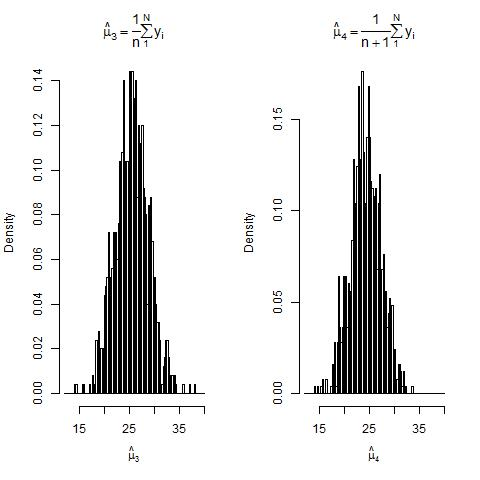
\includegraphics[width=\textwidth,height=3.125in]{./Fig/unbiasedness_vbig.jpg}
\caption{第三種與第四種樣本統計之模擬圖(樣本數=20)}
\end{figure}

\begin{figure}
\centering
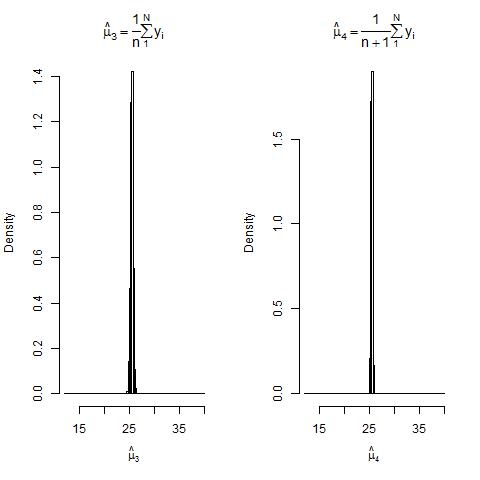
\includegraphics[width=\textwidth,height=3.125in]{./Fig/unbiasedness_vsmall.jpg}
\caption{第三種與第四種樣本統計之模擬圖(樣本數=2000)}
\end{figure}

\begin{itemize}
\item
  在樣本數趨近於無限大時,樣本統計的抽樣分佈會趨近於特定值。也就是變異數趨近於0。
\item
  \(\hat{\mu_{3}}\)是無偏且穩定之樣本統計,\(E[\hat{\mu_{3}}]=\mu\).
  \(\hat{\mu_{4}}\)是偏差但穩定之樣本統計。
\end{itemize}

\hypertarget{weak-law-of-large-numbers}{%
\subsubsection{Weak Law of Large
Numbers}\label{weak-law-of-large-numbers}}

弱大數法則:如果有\(X_{1}, X_{2},\cdots X_{n}\)等一系列的變數,彼此互相獨立,每依變數的平均數等於母體參數\(\mu\)。對\(\epsilon>0\),\(\bar{M_{n}}\)為平均數\(\frac{M_{1}+M_{2}+\cdots +M_{n}}{n}\)

當\(n\rightarrow \infty\)

\begin{center}
$Pr(|\bar{M_{n}}-\mu|\geq \epsilon)=\text{Pr}(|\frac{X_{1}+\cdots +X_{n}}{n}-\mu|\geq \epsilon)\rightarrow 0$
\end{center}

\begin{itemize}
\tightlist
\item
  以上的等式意義為當\(n\)趨近無限大,樣本平均數與母體平均數之間將沒有差異。
\item
  如果樣本數 \(n\) 夠大,那麼 \(M_{n}\) 的分佈將在 \(\mu\)
  的附近,或者是 \([\mu-\epsilon,\mu+\epsilon]\)這個區間
\item
  當\(n\rightarrow \infty\),樣本平均數會收斂於母體參數,也就是期望值。
\end{itemize}

\hypertarget{strong-law-of-large-numbers}{%
\subsubsection{Strong Law of Large
Numbers}\label{strong-law-of-large-numbers}}

強大數法則:如果有\(X_{1}, X_{2},\cdots X_{n}\)等一系列的變數,彼此互相獨立,母體參數為\(\mu\)。對\(\epsilon>0\),\(\bar{X_{n}}\)為平均數,則有以下結果:

\begin{center}
${\mathrm {lim}}_{n\rightarrow \infty}\text{Pr}(|\bar{X_{n}}-\mu|\geq \epsilon)=0$
\end{center}

或者是

\begin{center}
$Pr({\mathrm {lim}}_{n\rightarrow \infty}|\bar{X_{n}}=\mu)=1$\\
\end{center}

\begin{itemize}
\tightlist
\item
  強大數法則的意義為當\(n\rightarrow \infty\),樣本平均數等於母體參數的機率會收斂於1。
\end{itemize}

\hypertarget{ux6bcdux9ad4ux5e73ux5747ux6578ux7684ux4f30ux8a08}{%
\subsection{母體平均數的估計}\label{ux6bcdux9ad4ux5e73ux5747ux6578ux7684ux4f30ux8a08}}

\begin{itemize}
\tightlist
\item
  身高、體重、智商來自於常態分佈的母體,平均數為\(\bar{X}=\frac{X_{1}+\ldots+X_{n}}{n}\),機率分佈為\(f(X)=\frac{1}{\sigma\sqrt{2\pi}}\cdot e^{\frac{-(x-\mu)^2}{2\sigma^2}}\)。
\item
  \(\bar{X}\sim N(\mu, \frac{\sigma^2}{n})\)
\item
  \(\text{P}(\bar{X}-\mu \leq 1.96\sigma_{\bar{X}})=0.95\)
\end{itemize}

\hypertarget{ux6bcdux9ad4ux6bd4ux4f8bux7684ux4f30ux8a08}{%
\subsection{母體比例的估計}\label{ux6bcdux9ad4ux6bd4ux4f8bux7684ux4f30ux8a08}}

\begin{itemize}
\tightlist
\item
  在\(n\)次獨立重複伯努利試驗中,事件\(X\)發生的次數為
  \(n_{x}\)。\(\frac{n_{x}}{n}\)為事件\(X\)發生的機率事件\(X\)在每次試驗中發生的母體機率為\(p\)。對任意正數\(\epsilon>0\),以下等式成立:
\end{itemize}

\begin{center}
${\mathrm {lim}}_{n\rightarrow \infty}\text{Pr}(|\frac{n_{x}}{n}-p|< \epsilon)=1$
\end{center}

\begin{itemize}
\tightlist
\item
  強大數法則的意義為當\(n\rightarrow \infty\),樣本平均數等於母體參數的機率會收斂於1。請見圖3。
\end{itemize}

\begin{figure}
\centering
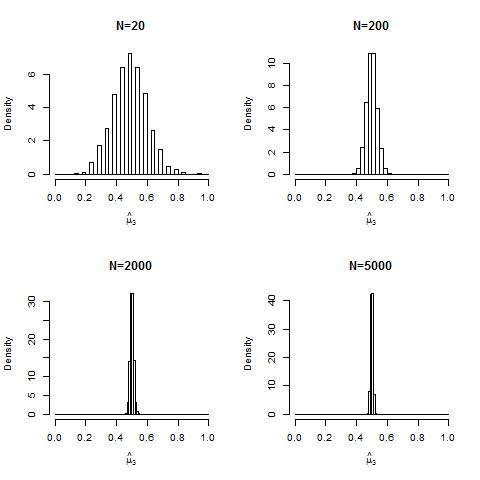
\includegraphics[width=\textwidth,height=3.125in]{./Fig/unbiasbinomial41.jpg}
\caption{二元變數之抽樣分佈模擬圖}
\end{figure}

\begin{itemize}
\item
  丟硬幣100次,其中得到52次正面、48次反面。我們對於母體的平均數估計是\(\frac{52}{100}\cdot 1+\frac{48}{100}\cdot 0=0.52\)。
\item
  如果我們相信母體平均數是0.52,那麼擲這枚硬幣10次,其中會得到6次正面的機率是:\(\frac{10!}{6!4!}(0.52)^6\cdot (1-0.52)^4=\)
\end{itemize}

\begin{Shaded}
\begin{Highlighting}[]
\NormalTok{p=}\FloatTok{0.52}\NormalTok{; n=}\DecValTok{10}\NormalTok{; x=}\DecValTok{6}
\NormalTok{(}\KeywordTok{factorial}\NormalTok{(n))}\OperatorTok{/}\NormalTok{(}\KeywordTok{factorial}\NormalTok{(x)}\OperatorTok{*}\KeywordTok{factorial}\NormalTok{(n}\OperatorTok{-}\NormalTok{x))}\OperatorTok{*}\NormalTok{p}\OperatorTok{^}\NormalTok{x}\OperatorTok{*}\NormalTok{(}\DecValTok{1}\OperatorTok{-}\NormalTok{p)}\OperatorTok{^}\DecValTok{4}
\CommentTok{## [1] 0.2203963}
\end{Highlighting}
\end{Shaded}

\begin{itemize}
\tightlist
\item
  假設我們抽樣100個同學,抽50次,而且我們相信女生佔了52\%,那麼這50套樣本當中,有多少套的樣本,女生剛好52人?
\end{itemize}

\begin{Shaded}
\begin{Highlighting}[]
\KeywordTok{set.seed}\NormalTok{(}\DecValTok{116}\NormalTok{)}
\NormalTok{m =}\StringTok{ }\DecValTok{50}\NormalTok{; n=}\StringTok{ }\DecValTok{100}\NormalTok{; p =}\StringTok{ }\FloatTok{.52}\NormalTok{;}
\NormalTok{phat =}\StringTok{ }\KeywordTok{rbinom}\NormalTok{(m,n,p)}\OperatorTok{/}\NormalTok{n}
\NormalTok{phat}
\CommentTok{##  [1] 0.48 0.51 0.50 0.58 0.51 0.57 0.50 0.57 0.58 0.55 0.54 0.53 0.54 0.54 0.51}
\CommentTok{## [16] 0.44 0.55 0.42 0.56 0.61 0.54 0.47 0.59 0.56 0.54 0.53 0.48 0.57 0.57 0.52}
\CommentTok{## [31] 0.60 0.45 0.48 0.62 0.52 0.59 0.52 0.56 0.51 0.57 0.63 0.51 0.57 0.48 0.44}
\CommentTok{## [46] 0.62 0.55 0.51 0.50 0.46}
\end{Highlighting}
\end{Shaded}

\begin{itemize}
\tightlist
\item
  我們排序50次的結果,然後以點狀圖表示:
\end{itemize}

\begin{Shaded}
\begin{Highlighting}[]
\KeywordTok{dotchart}\NormalTok{(}\KeywordTok{sort}\NormalTok{(phat), }\DataTypeTok{pch=}\DecValTok{16}\NormalTok{, }\DataTypeTok{col=}\StringTok{'#CCFF00'}\NormalTok{, }\DataTypeTok{yaxt=}\StringTok{'n'}\NormalTok{, }\DataTypeTok{xaxt=}\StringTok{'n'}\NormalTok{,   }
  \DataTypeTok{ylab=}\StringTok{''}\NormalTok{,}\DataTypeTok{xlab=}\KeywordTok{expression}\NormalTok{(}\KeywordTok{paste}\NormalTok{(}\StringTok{""}\NormalTok{, }\KeywordTok{hat}\NormalTok{(p))), }\DataTypeTok{cex.lab=}\FloatTok{1.8}\NormalTok{)}
\KeywordTok{abline}\NormalTok{(}\DataTypeTok{v =} \FloatTok{0.52}\NormalTok{, }\DataTypeTok{lwd=}\FloatTok{1.5}\NormalTok{, }\DataTypeTok{col=}\StringTok{'red3'}\NormalTok{, }\DataTypeTok{lty =} \DecValTok{2}\NormalTok{)}
\KeywordTok{mtext}\NormalTok{(}\StringTok{'0.52'}\NormalTok{,}\DecValTok{1}\NormalTok{)}
\end{Highlighting}
\end{Shaded}

\begin{figure}

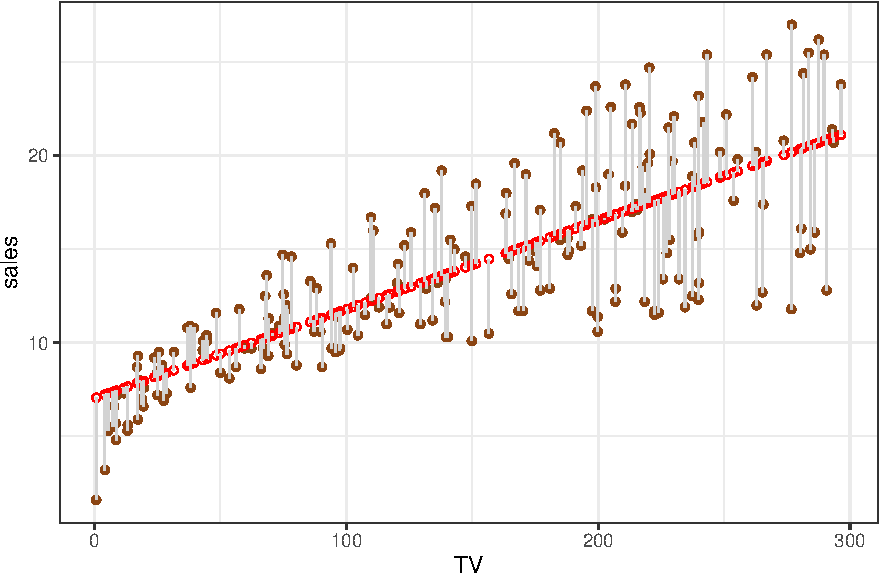
\includegraphics{Lec_test_05052020_files/figure-latex/unnamed-chunk-5-1} \hfill{}

\caption{\label{fig:dotchart1}二項分布抽樣之點狀圖}\label{fig:unnamed-chunk-5}
\end{figure}

\begin{itemize}
\tightlist
\item
  圖 \ref{fig:dotchart1}
  呈現出抽樣的結果,涵蓋小於0.45到大於0.6,但是只有幾個等於0.52。換句話說,抽樣得到的估計點,雖然理論上都是無偏估計,但是實際上與母體參數可能有一些不同。
\end{itemize}

\hypertarget{ux4e2dux592eux6975ux9650ux5b9aux7406}{%
\subsection{中央極限定理}\label{ux4e2dux592eux6975ux9650ux5b9aux7406}}

\begin{itemize}
\tightlist
\item
  有\(X_{1}, X_{2},\cdots X_{n}\)等一系列的變數,彼此互相獨立,母體參數為\(\mu\),
  \(\sigma^2<\infty\)時,對任何隨機變數的母體分佈下列公式成立:
\end{itemize}

\begin{center}
$\sqrt{n}(\bar{X_{n}}-\mu)\xrightarrow{d} N(0, \sigma^2)$
\end{center}

\begin{itemize}
\tightlist
\item
  \(n\)變大,\(\sqrt{n}\)倍的樣本平均數將會聚合在常態分佈。
\item
  因為\(Var[ax]=a^2Var[x]\),也就是對一個變數乘上\(a\)倍,它的變異數便是乘上\(a^2\)倍。所以
\end{itemize}

\begin{align*}
1/\sigma \cdot \sqrt{n}(\bar{X_{n}}-\mu)  \rightarrow 1/\sigma^2\cdot N(0, \sigma^2)=N(0,1)\\
\end{align*}

\begin{align}
\frac{1}{\sigma}\cdot \sqrt{n}(\bar{X_{n}}-\mu)\nonumber \\
& = \frac{\sqrt{n}(\bar{X_{n}}-\mu)}{\sigma}\nonumber \\
& = \frac{1/\sqrt{n}\cdot \sqrt{n}(\bar{X_{n}}-\mu)}{1/\sqrt{n}\cdot \sigma}\nonumber  \\
& =\frac{\bar{X_{n}}-\mu}{\frac{\sigma}{\sqrt{n}}}\label{eq:clt}
\end{align}

根據方程式(\ref{eq:clt})

\[Z_{n}\equiv \frac{\bar{X}_{n}-E[\bar{X}_{n}]}{\sqrt{V[\bar{X}_{n}]}}=\frac{\bar{X}_{n}-\mu}{\sigma/\sqrt{n}}\xrightarrow{d}{\mathit N}(0,1)\]

\begin{itemize}
\tightlist
\item
  中央極限定理可以應用到樣本統計(\(\bar{X}_{n}\))。
\item
  當\(n\)到一定規模時,標準化常態分佈(Standardized Normal
  Distribution)成立
\end{itemize}

\begin{center}
$\frac{|\bar{X}_{n}-\mu|}{\sigma/\sqrt{n}}\sim N(0,1)$
\end{center}

意謂著

\begin{center}
$\bar{X}_{n}\sim N(\mu,\sigma/\sqrt{n})$
\end{center}

\begin{itemize}
\item
  當樣本規模夠大時,不論是來自於哪一種分佈,樣本統計會形成常態分佈的抽樣分佈。
\item
  常態分佈的抽樣分佈可以用標準常態分佈表示,\(\text{Z}\sim \text{N}(0, 1)\)。我們用圖
  \ref{fig:ztwotail} 表示信賴水準0.95的區間:
\end{itemize}

\begin{figure}

\includegraphics{Lec_test_05052020_files/figure-latex/unnamed-chunk-6-1} \hfill{}

\caption{\label{fig:ztwotail}標準常態分佈信賴水準0.05的區間}\label{fig:unnamed-chunk-6}
\end{figure}

\begin{itemize}
\tightlist
\item
  圖 \ref{fig:ztwotail}
  顯示每一個Z值對應的機率密度。我們可以畫\(\text{Pr}(X\leq z)\)的累積機率圖如圖
  \ref{fig:zcum}。
\end{itemize}

\begin{Shaded}
\begin{Highlighting}[]
\KeywordTok{plot.new}\NormalTok{()}
\NormalTok{zx<-}\KeywordTok{seq}\NormalTok{(}\OperatorTok{-}\DecValTok{3}\NormalTok{, }\DecValTok{3}\NormalTok{, }\DataTypeTok{length.out=}\DecValTok{100}\NormalTok{)}
\KeywordTok{cat}\NormalTok{(}\StringTok{"P(Z=-3)="}\NormalTok{, }\KeywordTok{pnorm}\NormalTok{(zx[}\DecValTok{1}\NormalTok{], }\DecValTok{0}\NormalTok{, }\DecValTok{1}\NormalTok{),}\StringTok{"}\CharTok{\textbackslash{}n}\StringTok{"}\NormalTok{)}
\CommentTok{## P(Z=-3)= 0.001349898}
\KeywordTok{cat}\NormalTok{(}\StringTok{"P(Z=0)="}\NormalTok{, }\KeywordTok{pnorm}\NormalTok{(zx[}\DecValTok{50}\NormalTok{], }\DecValTok{0}\NormalTok{, }\DecValTok{1}\NormalTok{),}\StringTok{"}\CharTok{\textbackslash{}n}\StringTok{"}\NormalTok{)}
\CommentTok{## P(Z=0)= 0.4879127}
\KeywordTok{cat}\NormalTok{(}\StringTok{"P(Z=-3)="}\NormalTok{, }\KeywordTok{pnorm}\NormalTok{(zx[}\DecValTok{100}\NormalTok{], }\DecValTok{0}\NormalTok{, }\DecValTok{1}\NormalTok{))}
\CommentTok{## P(Z=-3)= 0.9986501}
\KeywordTok{plot}\NormalTok{(zx, }\KeywordTok{pnorm}\NormalTok{(zx, }\DecValTok{0}\NormalTok{, }\DecValTok{1}\NormalTok{), }\DataTypeTok{cex=}\FloatTok{0.3}\NormalTok{, }\DataTypeTok{col=}\StringTok{"#ea1021"}\NormalTok{)}
\KeywordTok{abline}\NormalTok{(}\DataTypeTok{h=}\KeywordTok{pnorm}\NormalTok{(zx[}\DecValTok{50}\NormalTok{], }\DecValTok{0}\NormalTok{, }\DecValTok{1}\NormalTok{), }\DataTypeTok{v=}\DecValTok{0}\NormalTok{ )}
\end{Highlighting}
\end{Shaded}

\begin{figure}

\includegraphics{Lec_test_05052020_files/figure-latex/unnamed-chunk-7-1} \hfill{}

\caption{\label{fig:zcum}Z值累積機率圖}\label{fig:unnamed-chunk-7}
\end{figure}

\begin{itemize}
\tightlist
\item
  二項分布指的是在\(n\)次的伯努力實驗中,如果用\(X\)隨機變數代表事件為真的次數,而且已知成功機率為\(p\),當\(X=k\)的機率是:\({n}\choose{k}\)
  \(\times p^{k}(1-p)^{n-k}\)。我們用圖 \ref{fig:pttwotail}
  表示當\(X\)從0到100而次數固定為100以及母體機率為0.5,對應的機率類似常態分佈,但是實際上這不是機率密度分佈,而是機率質量分佈,因為\(X\)並不是連續變數:
\end{itemize}

\begin{Shaded}
\begin{Highlighting}[]
\KeywordTok{plot.new}\NormalTok{()}
\NormalTok{k <-}\StringTok{ }\KeywordTok{c}\NormalTok{(}\DecValTok{0} \OperatorTok{:}\StringTok{ }\DecValTok{100}\NormalTok{)}
\NormalTok{size=}\DecValTok{100}\NormalTok{; pb=}\FloatTok{0.5}
\NormalTok{y <-}\StringTok{ }\KeywordTok{dbinom}\NormalTok{(k, }\DataTypeTok{size=}\NormalTok{size, }\DataTypeTok{prob=}\NormalTok{pb)}
\KeywordTok{plot}\NormalTok{(k, y,  }\DataTypeTok{xlab =} \StringTok{"count"}\NormalTok{, }\DataTypeTok{ylab =} \StringTok{"Pr(X=k)"}\NormalTok{, }\DataTypeTok{type=}\StringTok{"n"}\NormalTok{, }\DataTypeTok{main =} \StringTok{""}\NormalTok{)}
\KeywordTok{lines}\NormalTok{(k, y, }\DataTypeTok{col=}\StringTok{"#0011aa"}\NormalTok{)}
\end{Highlighting}
\end{Shaded}

\begin{figure}

\includegraphics{Lec_test_05052020_files/figure-latex/unnamed-chunk-8-1} \hfill{}

\caption{\label{fig:pbtwotail}二項分佈}\label{fig:unnamed-chunk-8}
\end{figure}

\begin{itemize}
\tightlist
\item
  圖 \ref{fig:pbcum}
  則是表示二項分佈\(\text{Pr}(X\leq k)\)的機率,也就是\(\sum_{x\leq k}\text{P}(X=k)\)的機率:
\end{itemize}

\begin{Shaded}
\begin{Highlighting}[]
\KeywordTok{plot.new}\NormalTok{()}
\NormalTok{k <-}\StringTok{ }\KeywordTok{c}\NormalTok{(}\DecValTok{0} \OperatorTok{:}\StringTok{ }\DecValTok{100}\NormalTok{)}
\NormalTok{size=}\DecValTok{100}\NormalTok{; pb=}\FloatTok{0.5}
\NormalTok{y <-}\StringTok{ }\KeywordTok{pbinom}\NormalTok{(k, }\DataTypeTok{size=}\NormalTok{size, }\DataTypeTok{prob=}\NormalTok{pb)}
\KeywordTok{plot}\NormalTok{(k, y,  }\DataTypeTok{xlab =} \StringTok{"count"}\NormalTok{, }\DataTypeTok{ylab =} \StringTok{"Pr(X=k)"}\NormalTok{, }\DataTypeTok{type=}\StringTok{"n"}\NormalTok{, }\DataTypeTok{main =} \StringTok{""}\NormalTok{)}
\KeywordTok{lines}\NormalTok{(k, y, }\DataTypeTok{col=}\StringTok{"#aa0022"}\NormalTok{)}
\end{Highlighting}
\end{Shaded}

\begin{figure}

\includegraphics{Lec_test_05052020_files/figure-latex/unnamed-chunk-9-1} \hfill{}

\caption{\label{fig:pbcum}二項分佈累積機率}\label{fig:unnamed-chunk-9}
\end{figure}

\hypertarget{ux4fe1ux8cf4ux5340ux9593}{%
\subsection{信賴區間}\label{ux4fe1ux8cf4ux5340ux9593}}

\begin{itemize}
\tightlist
\item
  雖然點估計是無偏估計,但是區間估計比點估計可靠。
\item
  區間估計需要考慮變數的平均數的變異程度,因為我們每次抽出的樣本所得到的平均數不會都相同,所以\(\bar{X}\)的變異數\(\sigma_{\bar{X}}\)的大小會影響區間估計。
\item
  區間的信賴水準(confidence
  level)以\(1-\alpha\)表示,\(\alpha=0.05\)時,代表信賴水準為0.95或者\(95\%\)。
\item
  因此,信賴區間是在一個既定信賴水準構成的區間,包含樣本統計量以及抽樣誤差。
\item
  步驟:
\end{itemize}

\begin{enumerate}
\def\labelenumi{\arabic{enumi}.}
\tightlist
\item
  選擇估計式、計算估計值
\item
  取得樣本統計量的抽樣分配,例如常態分配、t分配。在常態分佈而且信賴水準為\(95\%\)時,母體參數\(\mu\)與樣本平均值之間的差距,應該不會大於\(1.96*\sigma_{\bar{X}}\)。
\item
  得出母體參數的信賴區間
\item
  得出母體參數的結論
\end{enumerate}

\begin{itemize}
\tightlist
\item
  我們用區間估計表示抽樣的結果,也就是點估計加上一定的區間。
\end{itemize}

\begin{Shaded}
\begin{Highlighting}[]
\KeywordTok{set.seed}\NormalTok{(}\DecValTok{116}\NormalTok{)}
\NormalTok{m =}\StringTok{ }\DecValTok{50}\NormalTok{; n=}\StringTok{ }\DecValTok{100}\NormalTok{; p =}\StringTok{ }\FloatTok{.52}\NormalTok{;}
\NormalTok{phat =}\StringTok{ }\KeywordTok{rbinom}\NormalTok{(m,n,p)}\OperatorTok{/}\NormalTok{n}
\NormalTok{SE =}\StringTok{ }\KeywordTok{sqrt}\NormalTok{(phat}\OperatorTok{*}\NormalTok{(}\DecValTok{1}\OperatorTok{-}\NormalTok{phat)}\OperatorTok{/}\NormalTok{n)}
\NormalTok{alpha =}\StringTok{ }\FloatTok{0.05}\NormalTok{;zstar =}\StringTok{ }\KeywordTok{qnorm}\NormalTok{(}\DecValTok{1}\OperatorTok{-}\NormalTok{alpha}\OperatorTok{/}\DecValTok{2}\NormalTok{)}
\KeywordTok{cat}\NormalTok{(}\StringTok{"zstar="}\NormalTok{, zstar)}
\CommentTok{## zstar= 1.959964}
\KeywordTok{matplot}\NormalTok{(}\KeywordTok{rbind}\NormalTok{(phat }\OperatorTok{-}\StringTok{ }\NormalTok{zstar}\OperatorTok{*}\NormalTok{SE, phat }\OperatorTok{+}\StringTok{ }\NormalTok{zstar}\OperatorTok{*}\NormalTok{SE),}
  \KeywordTok{rbind}\NormalTok{(}\DecValTok{1}\OperatorTok{:}\NormalTok{m,}\DecValTok{1}\OperatorTok{:}\NormalTok{m), }\DataTypeTok{type=}\StringTok{"l"}\NormalTok{, }\DataTypeTok{lty=}\DecValTok{1}\NormalTok{,}
\DataTypeTok{xlab=}\KeywordTok{expression}\NormalTok{(}\KeywordTok{paste}\NormalTok{(}\KeywordTok{hat}\NormalTok{(p)}\OperatorTok{-}\NormalTok{z,}\StringTok{"*"}\NormalTok{,SE,}\StringTok{",  "}\NormalTok{, }\KeywordTok{hat}\NormalTok{(p)}\OperatorTok{+}\NormalTok{z,}\StringTok{"*"}\NormalTok{,SE)), }\DataTypeTok{ylab=}\StringTok{""}\NormalTok{)}
\KeywordTok{abline}\NormalTok{(}\DataTypeTok{v=}\NormalTok{p) }
\end{Highlighting}
\end{Shaded}

\begin{figure}

\includegraphics{Lec_test_05052020_files/figure-latex/unnamed-chunk-10-1} \hfill{}

\caption{\label{fig:interval1}區間估計圖}\label{fig:unnamed-chunk-10}
\end{figure}

這個圖 \ref{fig:interval1} 是由以下幾個參數所組成:

\begin{itemize}
\tightlist
\item
  \(\hat{p}\) 表示每一套樣本當中,女生的比例
\item
  SE表示樣本的標準誤=\(\sqrt{\frac{p(1-p)}{n}}\)
\item
  \(\alpha\)(alpha)表示我們估計時容許的抽樣誤差,也稱為顯著水準(significance
  level),顯著水準越小,代表誤判虛無假設成立的機會越小。一般設定為0.05或是\(5\%\),分成左右兩邊各是0.025
\item
  \(z^{*}\)表示一定的顯著水準下,對應的z值。顯著水準越大,z值越小。z值來自平均為0,變異數為1的分佈。
\item
  \(z^{*}\cdot SE\)表示一定顯著水準下,涵蓋母體參數的上下限。顯著水準越小、範圍越大、區間越容易涵蓋母體參數。
\item
  從這個圖可以看出,大部分的線跨過0.52這條垂直線,代表大部分抽樣的結果,涵蓋了母體為0.52這個參數。
\item
  因為區間估計比點估計來得周全,所以我們在檢定平均數或者平均數差異時,將使用區間估計。
\item
  標準誤表示為\(\frac{\sigma}{\sqrt{n}}\)。連續變數的\(\sigma\)的無偏估計是\(s=\frac{\sum(X_{i}-\bar{X})^2}{n-1}\)。二元變數則是\(\sqrt{p(1-p)}\)。
\end{itemize}

整理以上的資訊可以得到:

\begin{itemize}
\tightlist
\item
  \(\hat{p}\)的抽樣分配寫成:\(\hat{p}\sim N(p, \frac{p(1-p)}{n})\)。當\(\hat{p}=0.5\)時,\(\frac{p(1-p)}{n}\)會最大,也就是抽樣誤差會最大,避免低估所以如果我們不知道母體比例\(p\),可以先以\(\hat{p}=0.5\)代入。
\item
  利用\(Z\)分配求得\(\hat{p}\)與\(p\)的抽樣誤差為:\(\text{P}(|\hat{p}-p|\leq Z_{\alpha/2}\frac{p(1-p)}{n}) =1-\alpha\)
\item
  因此,母體比例\(p\)的信賴區間為:\([\hat{p}-Z_{\alpha/2}\frac{p(1-p)}{n}\leq p\leq \hat{p}+Z_{\alpha/2}\frac{p(1-p)}{n}]\)
\end{itemize}

\hypertarget{ux6bcdux9ad4ux5e73ux5747ux6578ux4e4bux5340ux9593ux4f30ux8a08ux8b8aux7570ux6578ux5df2ux77e5}{%
\subsubsection{母體平均數之區間估計(變異數已知)}\label{ux6bcdux9ad4ux5e73ux5747ux6578ux4e4bux5340ux9593ux4f30ux8a08ux8b8aux7570ux6578ux5df2ux77e5}}

\textbf{求取Z值} - 假設 Z 為標準常態分佈的隨機變數,請問 Z ≥ 1.27
的機率為多少?

\begin{Shaded}
\begin{Highlighting}[]
\KeywordTok{pnorm}\NormalTok{(}\FloatTok{1.27}\NormalTok{)}
\CommentTok{## [1] 0.8979577}
\DecValTok{1}\OperatorTok{-}\KeywordTok{pnorm}\NormalTok{(}\FloatTok{1.27}\NormalTok{)}
\CommentTok{## [1] 0.1020423}
\end{Highlighting}
\end{Shaded}

\textbf{平均睡眠時間}

\begin{itemize}
\item
  睡眠時間的平均值為6.5小時
\item
  標準差: 0.5小時
\item
  樣本數: 100
\item
  計算標準誤:
\end{itemize}

\[\sigma_{\bar{X}}=\frac{\sigma}{\sqrt{n}}=0.5/10=0.05\]

\begin{itemize}
\tightlist
\item
  因為在常態分佈而且信賴水準\(95\%\)時,\(|\bar{X}-\mu|\leq 1.96*\sigma_{\bar{X}}\),所以
\end{itemize}

\[|6.5-\mu|\leq 1.96*0.05=0.098\]

因為 \begin{equation*}
 |a-b|=
 \begin{cases}
 a-b & \text{if}\quad a-b\geq 0\\
 b-a & \text{if}\quad a-b\leq 0
 \end{cases}
\end{equation*}

所以 \begin{equation*}
 |6.5-\mu|=
 \begin{cases}
 6.5-\mu\leq 0.098 & 6.5-0.098=6.402\leq \mu \\
 \mu-6.5\leq 0.098 & \mu \leq 6.5+0.098=6.598
 \end{cases}
\end{equation*}

因此,睡眠的平均時間應該落在\(6.402\leq \mu \leq 6.598\)

\hypertarget{ux6bcdux9ad4ux6bd4ux4f8bux7684ux5340ux9593ux4f30ux8a08ux8b8aux7570ux6578ux672aux77e5}{%
\subsubsection{母體比例的區間估計(變異數未知)}\label{ux6bcdux9ad4ux6bd4ux4f8bux7684ux5340ux9593ux4f30ux8a08ux8b8aux7570ux6578ux672aux77e5}}

\begin{itemize}
\tightlist
\item
  樣本數: 1013
\item
  滿意政府的人數為466
\end{itemize}

\begin{enumerate}
\def\labelenumi{\arabic{enumi}.}
\tightlist
\item
  計算樣本比例:\(\hat{p}=466/1013=0.46\)
\item
  決定信賴水準:\(\alpha=0.05\)
\item
  \(z_{\alpha/2}=1.96\)
\end{enumerate}

\begin{Shaded}
\begin{Highlighting}[]
\NormalTok{alpha=}\FloatTok{0.05}
\NormalTok{zstar=}\OperatorTok{-}\KeywordTok{qnorm}\NormalTok{(alpha}\OperatorTok{/}\DecValTok{2}\NormalTok{)}
\KeywordTok{cat}\NormalTok{(}\StringTok{"z value="}\NormalTok{, zstar)}
\CommentTok{## z value= 1.959964}
\end{Highlighting}
\end{Shaded}

\begin{enumerate}
\def\labelenumi{\arabic{enumi}.}
\setcounter{enumi}{3}
\tightlist
\item
  95\%信賴區間:
\end{enumerate}

\begin{align*}
\hat{p}\pm 1.96\cdot \sqrt{\frac{0.46\cdot0.54}{1013}} & = 0.46\pm 1.96*0.015 \\
   & = 0.46\pm 0.03
\end{align*}

\begin{enumerate}
\def\labelenumi{\arabic{enumi}.}
\setcounter{enumi}{4}
\tightlist
\item
  結論:母體比例區間估計為 \((0.46-0.03\leq p\leq 0.46+0.03)\)
\end{enumerate}

\hypertarget{ux6a23ux672cux6578ux8207ux4fe1ux8cf4ux6c34ux6e96}{%
\subsubsection{樣本數與信賴水準}\label{ux6a23ux672cux6578ux8207ux4fe1ux8cf4ux6c34ux6e96}}

\begin{itemize}
\item
  因為 \(p=0.5\) 時,極大化標準誤
  \(\sqrt{\frac{p\cdot (1-p)}{n}}=\sqrt{0.25}{n}=\frac{0.5}{\sqrt{n}}\)
  。
\item
  如果信賴水準是0.95,\(z_{\alpha/2}\)經過查表或者計算,等於\(1.96\approx 2\),抽樣誤差等於\(z_{\alpha/2}*\sqrt{\frac{p\cdot (1-p)}{n}}\approx 2\cdot \frac{0.5}{n}=\frac{1}{\sqrt{n}}\)。
\item
  因此,我們通常用\(\frac{1}{\sqrt{n}}\)決定抽樣誤差,反過來,我們也可以先決定抽樣誤差,再來決定樣本數。
\end{itemize}

\hypertarget{tux5206ux4f48ux5340ux9593ux4f30ux8a08}{%
\subsection{t分佈區間估計}\label{tux5206ux4f48ux5340ux9593ux4f30ux8a08}}

雖然\(s\)是標準誤的無偏估計,但是\(s\)只是隨機亂數,並不是母體分佈。但是我們可以改用\(t\)分佈。\(t\)分布近似常態分佈,樣本數越大越接近常態分佈。

以下的圖顯示\(t\)分佈的自由度為1, 5, 10,
30時的機率分佈,\(t\)分佈的自由度是\(n-1\)。:

\begin{Shaded}
\begin{Highlighting}[]
\KeywordTok{curve}\NormalTok{(}\KeywordTok{dt}\NormalTok{(x, }\DecValTok{30}\NormalTok{), }\DataTypeTok{from =} \DecValTok{-5}\NormalTok{, }\DataTypeTok{to =} \DecValTok{5}\NormalTok{, }\DataTypeTok{col =} \StringTok{"orange"}\NormalTok{, }
      \DataTypeTok{xlab =} \StringTok{"quantile"}\NormalTok{, }\DataTypeTok{ylab =} \StringTok{"density"}\NormalTok{, }\DataTypeTok{lwd =} \DecValTok{2}\NormalTok{)}
\KeywordTok{curve}\NormalTok{(}\KeywordTok{dt}\NormalTok{(x, }\DecValTok{10}\NormalTok{), }\DataTypeTok{from =} \DecValTok{-5}\NormalTok{, }\DataTypeTok{to =} \DecValTok{5}\NormalTok{, }\DataTypeTok{col =} \StringTok{"green2"}\NormalTok{, }\DataTypeTok{add =} \OtherTok{TRUE}\NormalTok{, }\DataTypeTok{lwd =} \DecValTok{2}\NormalTok{)}
\KeywordTok{curve}\NormalTok{(}\KeywordTok{dt}\NormalTok{(x, }\DecValTok{5}\NormalTok{), }\DataTypeTok{from =} \DecValTok{-5}\NormalTok{, }\DataTypeTok{to =} \DecValTok{5}\NormalTok{, }\DataTypeTok{col =} \StringTok{"navyblue"}\NormalTok{, }\DataTypeTok{add =} \OtherTok{TRUE}\NormalTok{, }\DataTypeTok{lwd =} \DecValTok{2}\NormalTok{)}
\KeywordTok{curve}\NormalTok{(}\KeywordTok{dt}\NormalTok{(x, }\DecValTok{1}\NormalTok{), }\DataTypeTok{from =} \DecValTok{-5}\NormalTok{, }\DataTypeTok{to =} \DecValTok{5}\NormalTok{, }\DataTypeTok{col =} \StringTok{"grey40"}\NormalTok{, }\DataTypeTok{add =} \OtherTok{TRUE}\NormalTok{, }\DataTypeTok{lwd =} \DecValTok{2}\NormalTok{)}
\KeywordTok{legend}\NormalTok{(}\StringTok{"topleft"}\NormalTok{, }\DataTypeTok{legend =} \KeywordTok{paste0}\NormalTok{(}\StringTok{"DF = "}\NormalTok{, }\KeywordTok{c}\NormalTok{(}\DecValTok{1}\NormalTok{, }\DecValTok{5}\NormalTok{, }\DecValTok{10}\NormalTok{, }\DecValTok{30}\NormalTok{)),}
       \DataTypeTok{col =} \KeywordTok{c}\NormalTok{(}\StringTok{"grey40"}\NormalTok{, }\StringTok{"navyblue"}\NormalTok{, }\StringTok{"green2"}\NormalTok{, }\StringTok{"orange"}\NormalTok{),}
       \DataTypeTok{lty =} \DecValTok{1}\NormalTok{, }\DataTypeTok{lwd =} \DecValTok{2}\NormalTok{)}
\end{Highlighting}
\end{Shaded}

\begin{flushleft}\includegraphics{Lec_test_05052020_files/figure-latex/unnamed-chunk-13-1} \end{flushleft}

\begin{itemize}
\tightlist
\item
  \(t\)分佈形狀取決於自由度,自由度代表已知統計值之後,觀察值可以變動的數目。\(t\)分佈的形狀代表它的離散程度,或者是樣本變異數,而變異數來自於樣本平均值(\(\bar{X}\))。當我們已知平均值,只要有一個樣本不變,其他\(n-1\)個觀察值改變,還是可以得到相同的平均值。所以自由度是\(n-1\)。
\end{itemize}

以下的式子表示母體參數的上下區間的機率為\(1-\alpha\):

\[P(\bar{X}-t_{\alpha/2,n-1}S/\sqrt{n}<\mu<\bar{X}+t_{\alpha/2,n-1}S/\sqrt{n})=1-\alpha\]

\begin{itemize}
\tightlist
\item
  三種信賴區間的\(t\)值表示如表 \ref{tab:ttable2}:
  \textbackslash begin\{table\}
\end{itemize}

\caption{\label{tab:ttable2}三種信賴區間的t值}
\centering
\fontsize{14}{16}\selectfont
\begin{tabular}[t]{lrrrrr}
\toprule
信賴區間 & alpha & df.1 & df.4 & df.15 & df.3000\\
\midrule
90\% & 0.10 & 6.314 & 2.132 & 1.753 & 1.645\\
95\% & 0.05 & 12.710 & 2.776 & 2.131 & 1.960\\
99\% & 0.01 & 63.660 & 4.604 & 2.947 & 2.576\\
\bottomrule
\end{tabular}

\textbackslash end\{table\}

\begin{itemize}
\tightlist
\item
  \texttt{R}可以求得以上的機率,例如信賴區間為95\%時,\(\alpha\)除以2,加上自由度:
\end{itemize}

\begin{Shaded}
\begin{Highlighting}[]
\KeywordTok{qt}\NormalTok{(}\FloatTok{0.025}\NormalTok{, }\DecValTok{3000}\NormalTok{)}
\CommentTok{## [1] -1.960755}
\end{Highlighting}
\end{Shaded}

\begin{itemize}
\tightlist
\item
  \(t\)分佈的區間估計的步驟:
\end{itemize}

\hypertarget{ux7bc4ux4f8bux9ad4ux91cdux5e73ux5747ux503c}{%
\subsubsection{範例:體重平均值}\label{ux7bc4ux4f8bux9ad4ux91cdux5e73ux5747ux503c}}

\begin{itemize}
\tightlist
\item
  假設10位受試者的體重資料如下,請問平均體重等於173磅嗎?
\end{itemize}

\begin{Shaded}
\begin{Highlighting}[]
\NormalTok{weight <-}\KeywordTok{c}\NormalTok{(}\DecValTok{175}\NormalTok{, }\DecValTok{176}\NormalTok{, }\DecValTok{173}\NormalTok{, }\DecValTok{175}\NormalTok{, }\DecValTok{174}\NormalTok{, }\DecValTok{173}\NormalTok{, }\DecValTok{173}\NormalTok{, }\DecValTok{176}\NormalTok{, }\DecValTok{173}\NormalTok{, }\DecValTok{179}\NormalTok{)}
\KeywordTok{t.test}\NormalTok{(weight, }\DataTypeTok{mu=}\DecValTok{173}\NormalTok{)}
\CommentTok{## }
\CommentTok{##  One Sample t-test}
\CommentTok{## }
\CommentTok{## data:  weight}
\CommentTok{## t = 2.7618, df = 9, p-value = 0.02205}
\CommentTok{## alternative hypothesis: true mean is not equal to 173}
\CommentTok{## 95 percent confidence interval:}
\CommentTok{##  173.3076 176.0924}
\CommentTok{## sample estimates:}
\CommentTok{## mean of x }
\CommentTok{##     174.7}
\end{Highlighting}
\end{Shaded}

-分析顯示p-value \textless0.05,也就是說我們可以拒斥\(\mu=173\)的假設。
那麼我們要如何一步步計算\(T\)值以及\(t^{*}\)呢?

\begin{itemize}
\tightlist
\item
  先計算\(T\):
\end{itemize}

\begin{Shaded}
\begin{Highlighting}[]
\NormalTok{n=}\DecValTok{10}
\NormalTok{x_bar=}\KeywordTok{mean}\NormalTok{(weight)}
\NormalTok{s2=}\KeywordTok{sum}\NormalTok{((weight}\OperatorTok{-}\NormalTok{x_bar)}\OperatorTok{^}\DecValTok{2}\NormalTok{)}\OperatorTok{/}\NormalTok{(n}\DecValTok{-1}\NormalTok{)}
\NormalTok{c=}\DecValTok{173}
\NormalTok{T=(x_bar}\OperatorTok{-}\NormalTok{c)}\OperatorTok{/}\KeywordTok{sqrt}\NormalTok{(s2}\OperatorTok{/}\NormalTok{n)}
\NormalTok{T}
\CommentTok{## [1] 2.761805}
\end{Highlighting}
\end{Shaded}

已知\(T\)值,用pt(T, df)求p-value:

\begin{Shaded}
\begin{Highlighting}[]
\NormalTok{T=}\FloatTok{2.761805}
\NormalTok{pvalue=(}\DecValTok{1}\OperatorTok{-}\KeywordTok{pt}\NormalTok{(T, }\DataTypeTok{df=}\DecValTok{9}\NormalTok{))}\OperatorTok{*}\DecValTok{2}
\NormalTok{pvalue}
\CommentTok{## [1] 0.02204698}
\end{Highlighting}
\end{Shaded}

\begin{itemize}
\tightlist
\item
  之所以要先用1減pt(T,df)再除以2,是因為T對應的累積機率值是從最左邊一直累積過來,因此右邊的部分需要用1減。減完之後除以2代表左右兩邊各一半。
\item
  或者比較\(T\)與\(t^{*}\)
\end{itemize}

\begin{Shaded}
\begin{Highlighting}[]
\NormalTok{T=}\FloatTok{2.761805}
\NormalTok{t.star=}\KeywordTok{qt}\NormalTok{(}\FloatTok{0.975}\NormalTok{, }\DecValTok{9}\NormalTok{)}
\NormalTok{T}\OperatorTok{-}\NormalTok{t.star}
\CommentTok{## [1] 0.4996478}
\end{Highlighting}
\end{Shaded}

我們用圖 \ref{fig:twotail1} 表示信賴水準0.05的區間:

\begin{figure}

\includegraphics{Lec_test_05052020_files/figure-latex/unnamed-chunk-19-1} \hfill{}

\caption{\label{fig:twotail1}顯著水準0.05的區間}\label{fig:unnamed-chunk-19}
\end{figure}

圖
\ref{fig:twotail1}顯示,如果T=-1.98或者1.98,只有\(\frac{1-0.95}{2}=0.025\)的機率會發生。當T=2.76,右邊的區域剩下非常小的區域,換句話說,要觀察到T=2.76的機率非常小,如圖
\ref{fig:tvaluesmall}:

\begin{Shaded}
\begin{Highlighting}[]
\NormalTok{scale <-}\StringTok{ }\FloatTok{0.1} 
\NormalTok{x <-}\StringTok{ }\KeywordTok{seq}\NormalTok{(}\OperatorTok{-}\DecValTok{4}\NormalTok{, }\DecValTok{4}\NormalTok{, scale) }
\NormalTok{df=}\DecValTok{100}
\NormalTok{y <-}\StringTok{ }\KeywordTok{dt}\NormalTok{(x, df) }
\KeywordTok{plot}\NormalTok{(x, y, }\DataTypeTok{type =} \StringTok{"l"}\NormalTok{, }\DataTypeTok{main=}\StringTok{"t-Test, t = 2.76"}\NormalTok{) }

\NormalTok{linepos <-}\StringTok{ }\FloatTok{2.76} 
\KeywordTok{abline}\NormalTok{(}\DataTypeTok{v =}\NormalTok{ linepos) }
\NormalTok{cutpoint <-}\StringTok{ }\NormalTok{(}\KeywordTok{max}\NormalTok{(x) }\OperatorTok{-}\StringTok{ }\NormalTok{linepos) }\OperatorTok{/}\StringTok{ }\NormalTok{scale }

\NormalTok{xt <-}\StringTok{ }\NormalTok{x[(}\KeywordTok{length}\NormalTok{(x)}\OperatorTok{-}\NormalTok{cutpoint)}\OperatorTok{:}\KeywordTok{length}\NormalTok{(x)] }
\NormalTok{yt <-}\StringTok{ }\NormalTok{y[(}\KeywordTok{length}\NormalTok{(y)}\OperatorTok{-}\NormalTok{cutpoint)}\OperatorTok{:}\KeywordTok{length}\NormalTok{(y)] }

\CommentTok{# draw the polygon }

\NormalTok{n <-}\StringTok{ }\KeywordTok{length}\NormalTok{(xt) }
\NormalTok{xt <-}\StringTok{ }\KeywordTok{c}\NormalTok{(xt[}\DecValTok{1}\NormalTok{], xt, xt[n]) }
\NormalTok{yt <-}\StringTok{ }\KeywordTok{c}\NormalTok{(}\DecValTok{0}\NormalTok{,yt,}\DecValTok{0}\NormalTok{) }
\KeywordTok{polygon}\NormalTok{(xt, yt, }\DataTypeTok{col=}\StringTok{"red"}\NormalTok{ ) }
\end{Highlighting}
\end{Shaded}

\begin{figure}

\includegraphics{Lec_test_05052020_files/figure-latex/unnamed-chunk-20-1} \hfill{}

\caption{\label{fig:tvaluesmall}T值等於2.76}\label{fig:unnamed-chunk-20}
\end{figure}

\begin{itemize}
\tightlist
\item
  T值對應的機率在曲線底下的面積是1,因此T值對應的機率可以用累積機率的方式呈現如圖
  \ref{fig:cumu1}。當T=-3時,累積機率為0.0026或者0.26\%,而到了T=0的累積機率則是0.5,T=3時,就是累積機率等於1。
\end{itemize}

\begin{Shaded}
\begin{Highlighting}[]
\NormalTok{tx<-}\KeywordTok{seq}\NormalTok{(}\OperatorTok{-}\DecValTok{3}\NormalTok{, }\DecValTok{3}\NormalTok{, }\DataTypeTok{length.out=}\DecValTok{100}\NormalTok{)}
\KeywordTok{cat}\NormalTok{(}\StringTok{"P(T=-3)="}\NormalTok{,}\KeywordTok{pt}\NormalTok{(tx[}\DecValTok{1}\NormalTok{], }\DataTypeTok{df=}\DecValTok{30}\NormalTok{),}\StringTok{"}\CharTok{\textbackslash{}n}\StringTok{"}\NormalTok{)}
\CommentTok{## P(T=-3)= 0.002694982}
\KeywordTok{cat}\NormalTok{(}\StringTok{"P(T=0)="}\NormalTok{,}\KeywordTok{pt}\NormalTok{(tx[}\DecValTok{50}\NormalTok{], }\DataTypeTok{df=}\DecValTok{30}\NormalTok{),}\StringTok{"}\CharTok{\textbackslash{}n}\StringTok{"}\NormalTok{)}
\CommentTok{## P(T=0)= 0.488013}
\KeywordTok{cat}\NormalTok{(}\StringTok{"P(T=-3)="}\NormalTok{, }\KeywordTok{pt}\NormalTok{(tx[}\DecValTok{100}\NormalTok{], }\DataTypeTok{df=}\DecValTok{30}\NormalTok{))}
\CommentTok{## P(T=-3)= 0.997305}
\KeywordTok{plot}\NormalTok{(tx, }\KeywordTok{pt}\NormalTok{(tx, }\DataTypeTok{df=}\DecValTok{30}\NormalTok{), }\DataTypeTok{cex=}\FloatTok{0.3}\NormalTok{, }\DataTypeTok{col=}\StringTok{"sandybrown"}\NormalTok{)}
\end{Highlighting}
\end{Shaded}

\begin{figure}

\includegraphics{Lec_test_05052020_files/figure-latex/unnamed-chunk-21-1} \hfill{}

\caption{\label{fig:cumu1}t分佈累積機率圖}\label{fig:unnamed-chunk-21}
\end{figure}

\hypertarget{ux5047ux8a2dux6aa2ux5b9a}{%
\section{假設檢定}\label{ux5047ux8a2dux6aa2ux5b9a}}

\begin{itemize}
\tightlist
\item
  假設檢定與區間估計的原理相同,但是假設檢定多了建立假設以及驗證假設的步驟,例如我們要檢定某個樣本估計值是否等於特定常數,步驟如下:
\end{itemize}

\begin{enumerate}
\def\labelenumi{\arabic{enumi}.}
\item
  假設\(\mu=c\)。
\item
  決定顯著水準\(\alpha\)或者信賴區間\((1-\alpha)\%\)
\item
  計算自由度\(n-1\)
\item
  計算\(T=\frac{X-c}{s/\sqrt{n}}\)
\item
  計算顯著水準\(\alpha\)與自由度相對應的\(t^{*}\)值。\(\alpha=5\%\)、自由度等於1,000時,約為1.962
\end{enumerate}

\begin{Shaded}
\begin{Highlighting}[]
\KeywordTok{qt}\NormalTok{(}\FloatTok{0.975}\NormalTok{, }\DecValTok{1000}\NormalTok{)}
\CommentTok{## [1] 1.962339}
\end{Highlighting}
\end{Shaded}

\begin{enumerate}
\def\labelenumi{\arabic{enumi}.}
\setcounter{enumi}{5}
\item
  當\(p(T)<\alpha\),表示會發生c的機會非常小,可以拒斥\(\mu=c\)的假設。
\item
  同樣的當\(T>t_{*}\),表示會發生c的機會非常小,可以拒斥\(\mu=c\)的假設。
\end{enumerate}

\begin{itemize}
\tightlist
\item
  由以上步驟可知,假設檢定涉及到樣本估計值與欲檢驗值的差距,以及樣本估計的變異程度,還有信賴水準的大小。
\end{itemize}

\hypertarget{ux96d9ux5c3eux6aa2ux5b9aux865bux7121ux5047ux8a2dux8207ux5c0dux7acbux5047ux8a2d}{%
\subsection{雙尾檢定虛無假設與對立假設}\label{ux96d9ux5c3eux6aa2ux5b9aux865bux7121ux5047ux8a2dux8207ux5c0dux7acbux5047ux8a2d}}

\begin{itemize}
\item
  虛無假設:假設母體參數或者其他參數為真,除非證明非真。寫成\(H_{\text{0}}\)。
  例如\(H_{\text{0}}: \mu = 0\).
\item
  對立假設:相對於虛無假設,提出不同的假設,寫成\(H_{\text{1}}\)。例如\(H_{\text{1}}: \mu \neq 0\).
\item
  假設樣本來自於常態分佈,而且抽取時互相獨立,樣本估計值除以標準誤之後形成常態分佈,因此樣本估計值與虛無假設中的母體參數之間的差距,除以標準誤之後,我們可以檢驗\(T\)值是否大於樣本分佈的特定信賴水準的臨界點\(t^{*}\)。如果大於臨界點,表示要觀察到這樣的差距的機會很小,也就是我們可以說這樣的差距統計上很顯著。換句話說,我們可以下結論說樣本估計值並不會等於虛無假設中的參數,我們不接受虛無假設。
\item
  反過來說,如果小於臨界點,表示很容易觀察到這樣的差距,也就是兩者之間沒有差距的機會很大,所以結論是虛無假設成立。
\item
  圖 \ref{fig:accept} 顯示接受域以及拒斥域。
\end{itemize}

\begin{figure}

\includegraphics{Lec_test_05052020_files/figure-latex/acceptarea-1} \hfill{}

\caption{\label{fig:accept}拒絕域與接受域}\label{fig:acceptarea}
\end{figure}

\hypertarget{ux6aa2ux9a57ux5047ux8a2dux7d50ux679c}{%
\subsection{檢驗假設結果}\label{ux6aa2ux9a57ux5047ux8a2dux7d50ux679c}}

\begin{itemize}
\tightlist
\item
  Type I error:
  當\(H_{\text{0}}\)為真,但是拒絕\(H_{\text{0}}\)。以\(\alpha\)表示:
\end{itemize}

\[\alpha=\text{Pr}(\text{reject}\hspace{.2em}H_{\text{0}}|H_{\text{0}}\hspace{.2em} \text{is}\hspace{.2em} \text{true})\]

\begin{itemize}
\tightlist
\item
  Type II error:
  當\(H_{\text{0}}\)為偽,但是沒有拒絕\(H_{\text{0}}\)。以\(\beta\)表示:
\end{itemize}

\[\beta=\text{Pr}(\text{not reject}\hspace{.2em}H_{\text{0}}|H_{\text{0}}\hspace{.2em} \text{is}\hspace{.2em} \text{false})\]

\begin{itemize}
\tightlist
\item
  圖 \ref{fig:twotailleft}
  顯示左側有\(\alpha=0.05\)的拒斥區域。當\(H_{\text{0}}: \mu=\mu_{0}\)為真,我們卻拒絕這個假設,我們犯錯的機率為\(\alpha\)。而且當\(H_{\text{0}}: \mu\geq \mu_{0}\)為真,我們卻拒絕這個假設,我們犯錯的機率也是\(\alpha\)。
\end{itemize}

\begin{figure}

\includegraphics{Lec_test_05052020_files/figure-latex/TypeI-1} \hfill{}

\caption{\label{fig:twotailleft}第一型錯誤}\label{fig:TypeI}
\end{figure}

\begin{itemize}
\tightlist
\item
  圖 \ref{fig:twotailright}
  顯示右側有\(\beta\)的拒斥區域。當\(H_{\text{0}}: \mu=\mu_{0}\)不為真,我們卻接受這個假設,我們犯錯的機率為\(\beta\)。而且當\(H_{\text{0}}: \mu\leq \mu_{0}\)不為真,我們卻接受這個假設,我們犯錯的機率也是\(\beta\)。
\end{itemize}

\begin{figure}

\includegraphics{Lec_test_05052020_files/figure-latex/type2-1} \hfill{}

\caption{\label{fig:twotailright}第二型錯誤}\label{fig:type2}
\end{figure}

\begin{itemize}
\tightlist
\item
  雙尾檢定的虛無假設是:
\end{itemize}

\[\text{H}_{\text{0}}: \mu = \mu_{0}\]

\begin{itemize}
\tightlist
\item
  而對立假設則是:
\end{itemize}

\[\text{H}_{\text{1}}: \mu \neq \mu_{0}\]

\hypertarget{ux7bc4ux4f8b}{%
\subsubsection{範例}\label{ux7bc4ux4f8b}}

\begin{itemize}
\item
  目前台灣的女性受雇員工的全年總薪資中位數約為45.6萬。調查一家公司,假設樣本數為102人,其中超過45.6萬的女性員工是54人,請問該公司女性員工年薪超過45.6萬的比例是否為\(p=0.5\)?
\item
  因為伯努利分佈的樣本變異數是\(p(1-p)\),所以樣本標準誤的公式為:
\end{itemize}

\(SE=\sqrt{\hat{p}(1-\hat{p})/n}\)

T值的公式為:

\(T=\frac{\hat{p}-c}{\sqrt{\hat{p}(1-\hat{p})/n}}\)

\begin{itemize}
\tightlist
\item
  我們用\texttt{R}計算並且檢定:
\end{itemize}

\begin{Shaded}
\begin{Highlighting}[]
\NormalTok{n=}\DecValTok{102}
\NormalTok{p=}\DecValTok{54}\OperatorTok{/}\DecValTok{102}
\NormalTok{c=}\FloatTok{0.5}
\NormalTok{T=(p}\OperatorTok{-}\NormalTok{c)}\OperatorTok{/}\KeywordTok{sqrt}\NormalTok{(p}\OperatorTok{*}\NormalTok{(}\DecValTok{1}\OperatorTok{-}\NormalTok{p)}\OperatorTok{/}\NormalTok{n)}
\NormalTok{T}
\CommentTok{## [1] 0.595119}
\end{Highlighting}
\end{Shaded}

\begin{itemize}
\tightlist
\item
  輸入T值,計算對應的p值:
\end{itemize}

\begin{Shaded}
\begin{Highlighting}[]
\NormalTok{T=}\FloatTok{0.595}\NormalTok{; n=}\DecValTok{102}
\NormalTok{pvalue=}\StringTok{ }\KeywordTok{pt}\NormalTok{(T, }\DataTypeTok{df=}\NormalTok{n}\DecValTok{-1}\NormalTok{, }\DataTypeTok{lower.tail =}\NormalTok{ F)}
\NormalTok{pvalue}
\CommentTok{## [1] 0.2765871}
\end{Highlighting}
\end{Shaded}

\begin{itemize}
\tightlist
\item
  因為p值大於0.05,所以我們的樣本可能來自於\(p=0.5\)的母體。
\end{itemize}

\begin{figure}
\centering
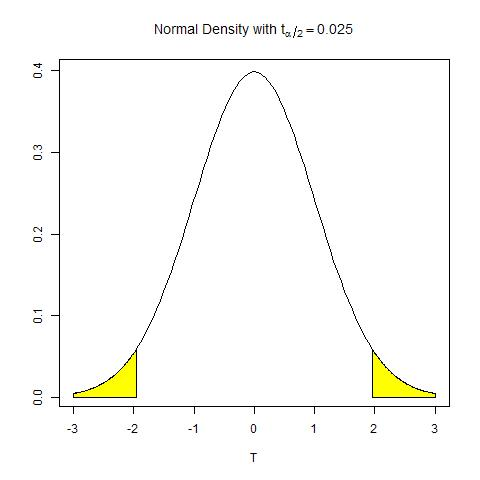
\includegraphics[width=\textwidth,height=3.125in]{./Fig/t_alpha1.jpg}
\caption{雙尾檢定圖}
\end{figure}

\begin{itemize}
\tightlist
\item
  我們也可用 \(\tt{prop.test()}\) 計算區間以及檢定(\(\tt{t.test()}\)
  需要原始資料):
\end{itemize}

\begin{Shaded}
\begin{Highlighting}[]
\KeywordTok{prop.test}\NormalTok{(}\DecValTok{54}\NormalTok{, }\DecValTok{102}\NormalTok{, }\DataTypeTok{p=}\FloatTok{0.5}\NormalTok{, }\DataTypeTok{conf.level=}\FloatTok{0.95}\NormalTok{)}
\CommentTok{## }
\CommentTok{##  1-sample proportions test with continuity correction}
\CommentTok{## }
\CommentTok{## data:  54 out of 102, null probability 0.5}
\CommentTok{## X-squared = 0.2451, df = 1, p-value = 0.6205}
\CommentTok{## alternative hypothesis: true p is not equal to 0.5}
\CommentTok{## 95 percent confidence interval:}
\CommentTok{##  0.4284751 0.6281074}
\CommentTok{## sample estimates:}
\CommentTok{##         p }
\CommentTok{## 0.5294118}
\end{Highlighting}
\end{Shaded}

\begin{itemize}
\item
  因為p-value\textgreater0.05,因此我們可以接受\(c=0.5\)的假設。換句話說,這一套樣本來自於\(p=0.5\)的母體。
\item
  由於\texttt{R}的
  \(\tt{prop.test()}\)用Z值與T值相比,所以p-value會與自行運算的結果不太相同。
\item
  輸入T值,改用標準常態分佈計算對應的p值:
\end{itemize}

\begin{Shaded}
\begin{Highlighting}[]
\NormalTok{T=}\FloatTok{0.595}
\NormalTok{pvalue=}\StringTok{ }\KeywordTok{pnorm}\NormalTok{(T, }\DecValTok{0}\NormalTok{, }\DecValTok{1}\NormalTok{)}
\NormalTok{pvalue}
\CommentTok{## [1] 0.7240783}
\end{Highlighting}
\end{Shaded}

\begin{itemize}
\tightlist
\item
  因為當T=0.5時,\(p\)值約為0.69,所以當T接近0.6時,\(p\)值也隨之增加。
\item
  雙尾檢定
\end{itemize}

\begin{Shaded}
\begin{Highlighting}[]
\NormalTok{n=}\DecValTok{102}\NormalTok{; }\KeywordTok{set.seed}\NormalTok{(}\DecValTok{02138}\NormalTok{)}
\NormalTok{upper=}\KeywordTok{prop.test}\NormalTok{(}\DecValTok{54}\NormalTok{, }\DecValTok{102}\NormalTok{, }\DataTypeTok{p=}\FloatTok{0.5}\NormalTok{, }\DataTypeTok{conf.level=}\FloatTok{0.95}\NormalTok{)}\OperatorTok{$}\NormalTok{conf.int[}\DecValTok{2}\NormalTok{]}
\NormalTok{lower=}\KeywordTok{prop.test}\NormalTok{(}\DecValTok{54}\NormalTok{, }\DecValTok{102}\NormalTok{, }\DataTypeTok{p=}\FloatTok{0.5}\NormalTok{, }\DataTypeTok{conf.level=}\FloatTok{0.95}\NormalTok{)}\OperatorTok{$}\NormalTok{conf.int[}\DecValTok{1}\NormalTok{]}
\KeywordTok{tibble}\NormalTok{(}\DataTypeTok{x=}\KeywordTok{rnorm}\NormalTok{(}\DecValTok{200}\NormalTok{, }\FloatTok{0.52}\NormalTok{, }\FloatTok{0.05}\NormalTok{)) }\OperatorTok
\StringTok{  }\KeywordTok{ggplot}\NormalTok{(}\KeywordTok{aes}\NormalTok{(}\DataTypeTok{x=}\NormalTok{x)) }\OperatorTok{+}
\StringTok{  }\KeywordTok{geom_histogram}\NormalTok{(}\DataTypeTok{fill=}\StringTok{'gray90'}\NormalTok{) }\OperatorTok{+}
\StringTok{  }\KeywordTok{geom_density}\NormalTok{(}\DataTypeTok{col=}\StringTok{'#0011EE'}\NormalTok{) }\OperatorTok{+}
\StringTok{  }\KeywordTok{geom_vline}\NormalTok{(}\DataTypeTok{xintercept =} \KeywordTok{c}\NormalTok{(lower, upper), }\DataTypeTok{lty=}\DecValTok{2}\NormalTok{, }\DataTypeTok{col=}\StringTok{"#EE00AA"}\NormalTok{) }\OperatorTok{+}
\StringTok{  }\KeywordTok{geom_vline}\NormalTok{(}\DataTypeTok{xintercept =} \FloatTok{0.52}\NormalTok{, }\DataTypeTok{lty=}\DecValTok{1}\NormalTok{, }\DataTypeTok{col=}\StringTok{"#AA1100"}\NormalTok{) }\OperatorTok{+}
\StringTok{  }\KeywordTok{theme_bw}\NormalTok{()}
\CommentTok{## `stat_bin()` using `bins = 30`. Pick better value with `binwidth`.}
\end{Highlighting}
\end{Shaded}

\begin{flushleft}\includegraphics{Lec_test_05052020_files/figure-latex/unnamed-chunk-27-1} \end{flushleft}

\hypertarget{ux55aeux5c3eux6aa2ux5b9a}{%
\subsubsection{單尾檢定}\label{ux55aeux5c3eux6aa2ux5b9a}}

\begin{itemize}
\item
  有時候我們需要檢定樣本平均數是否大於或者小於某一個數。例如學生的平均身高是否高於160公分,或者BMI值是否低於24。這時候我們可以用單尾檢定。單尾檢定需要把拒斥的區域集中在其中一邊,例如圖
  \ref{fig:onetail1}表示拒斥區域在左尾,這是我們假設母體參數大於假設值,除非我們發現用來推論母體的樣本統計值非常小,小到落在拒斥區域,那麼我們就不接受母體參數大於假設值,也就是母體參數其實小於假設值。如果顯著水準為0.05,那麼就是右邊0.05或是左邊0.05,而不是0.025。可以想像顯著水準0.05除以2所對應的\(t^{*}\)
  要比0.05對應的\(t^{*}\)來的大。
\item
  左尾檢定的虛無假設是:
\end{itemize}

\[\text{H}_{\text{0}}: \mu\geq \mu_{0}\]

\begin{itemize}
\tightlist
\item
  而對立假設則是:
\end{itemize}

\[\text{H}_{\text{1}}: \mu < \mu_{0}\]

\begin{itemize}
\item
  也可以詮釋成當我們用平均值\(\mu_{0}\)來隨機抽樣,要抽到\(<\mu_{0}\)(左尾)或是\(>\mu_{0}\)(右尾)的樣本的機會是\(p\)值。如果\(p\)小於5\%,那麼我們可以說機會非常小,無法接受虛無假設成立。所以結論是我們可以接受對立假設,也就是\(\mu>\mu_{0}\)(左尾)或是\(\mu < \mu_{0}\)(右尾)。
\item
  例如過去研究宣稱某種病毒在人體表面可以生存超過5天,不管是6天、10天都比5天來得長。雖然我們懷疑這個研究發現過度誇大病毒的存活能力,但是我們除非發現的樣本統計值,換算成Z值或者t值之後小於臨界值,那麼我們才會推翻虛無假設。但是如果Z值或者t值大於臨界值,不論有多大,都符合虛無假設。
\item
  通常我們設定的標準是5\%,要小於這個標準我們才拒斥虛無假設,也就是我們已經有點相信虛無假設,除非我們發現很有力的證據才能推翻虛無假設。
\end{itemize}

\begin{Shaded}
\begin{Highlighting}[]
\KeywordTok{plot.new}\NormalTok{()}
\NormalTok{x <-}\StringTok{ }\KeywordTok{seq}\NormalTok{(}\OperatorTok{-}\DecValTok{4}\NormalTok{, }\DecValTok{4}\NormalTok{, }\DataTypeTok{length =} \DecValTok{1000}\NormalTok{)}
\NormalTok{y <-}\StringTok{ }\KeywordTok{dnorm}\NormalTok{(x, }\DecValTok{0}\NormalTok{, }\DecValTok{1}\NormalTok{)}
\KeywordTok{plot}\NormalTok{(x, y, }\DataTypeTok{type=}\StringTok{"n"}\NormalTok{, }\DataTypeTok{xlab =} \StringTok{""}\NormalTok{, }\DataTypeTok{ylab =} \StringTok{""}\NormalTok{, }\DataTypeTok{main =} \StringTok{""}\NormalTok{, }\DataTypeTok{axes =} \OtherTok{FALSE}\NormalTok{)}
\KeywordTok{axis}\NormalTok{(}\DecValTok{1}\NormalTok{)}
\KeywordTok{lines}\NormalTok{(x, y)}

\NormalTok{alpha=}\FloatTok{0.05}
\NormalTok{lower_bound <-}\StringTok{ }\DecValTok{0}\OperatorTok{-}\KeywordTok{qnorm}\NormalTok{(}\DecValTok{1}\OperatorTok{-}\NormalTok{alpha, }\DecValTok{0}\NormalTok{, }\DecValTok{1}\NormalTok{)}
\NormalTok{upper_bound <-}\StringTok{ }\DecValTok{0}\OperatorTok{+}\KeywordTok{qnorm}\NormalTok{(}\DecValTok{1}\OperatorTok{-}\NormalTok{alpha, }\DecValTok{0}\NormalTok{, }\DecValTok{1}\NormalTok{)}
\NormalTok{bounds_filter <-}\StringTok{ }\NormalTok{x }\OperatorTok{>=}\StringTok{ }\DecValTok{-4} \OperatorTok{&}\StringTok{ }\NormalTok{x }\OperatorTok{<=}\StringTok{ }\NormalTok{lower_bound}
\NormalTok{x_within_bounds <-}\StringTok{ }\NormalTok{x[bounds_filter]}
\NormalTok{y_within_bounds <-}\StringTok{ }\NormalTok{y[bounds_filter]}
 
\NormalTok{x_polygon <-}\StringTok{ }\KeywordTok{c}\NormalTok{(}\OperatorTok{-}\DecValTok{4}\NormalTok{, x_within_bounds, lower_bound)}
\NormalTok{y_polygon <-}\StringTok{ }\KeywordTok{c}\NormalTok{(}\DecValTok{0}\NormalTok{, y_within_bounds, }\DecValTok{0}\NormalTok{)}
 
\KeywordTok{polygon}\NormalTok{(x_polygon, y_polygon, }\DataTypeTok{col =} \StringTok{"red"}\NormalTok{)}
\KeywordTok{text}\NormalTok{(}\OperatorTok{-}\FloatTok{2.6}\NormalTok{, }\FloatTok{0.1}\NormalTok{, }\KeywordTok{expression}\NormalTok{(}\KeywordTok{paste}\NormalTok{(}\KeywordTok{bold}\NormalTok{(alpha))))}
\KeywordTok{segments}\NormalTok{(}\OperatorTok{-}\FloatTok{2.6}\NormalTok{, }\FloatTok{0.09}\NormalTok{, }\FloatTok{-2.2}\NormalTok{, }\FloatTok{0.02}\NormalTok{, }\DataTypeTok{lty=}\DecValTok{2}\NormalTok{)}
\KeywordTok{segments}\NormalTok{(}\DecValTok{0}\NormalTok{, }\DecValTok{0}\NormalTok{, }\DecValTok{0}\NormalTok{, }\FloatTok{0.4}\NormalTok{, }\DataTypeTok{lty=}\DecValTok{2}\NormalTok{)}
\end{Highlighting}
\end{Shaded}

\begin{figure}

\includegraphics{Lec_test_05052020_files/figure-latex/lefttail-1} \hfill{}

\caption{\label{fig:onetail1}左尾檢定圖}\label{fig:lefttail}
\end{figure}

\begin{itemize}
\item
  反之,如果我們想要檢定平均數大於\(\mu_{0}\),那麼可以採用右尾檢定,也就是如果我們觀察到的樣本估計值非常大,大到母體平均數很難超過它,那麼我們可以拒斥平均值小於\(\mu_{0}\)的虛無假設,也就是接受大於\(\mu_{0}\)的對立假設。
\item
  右尾檢定的虛無假設是:
\end{itemize}

\[\text{H}_{\text{0}}: \mu\leq \mu_{0}\]

\begin{itemize}
\tightlist
\item
  而對立假設則是:
\end{itemize}

\[\text{H}_{\text{1}}: \mu > \mu_{0}\] - 下圖表示右側的區域為0.05。

\begin{figure}
\centering
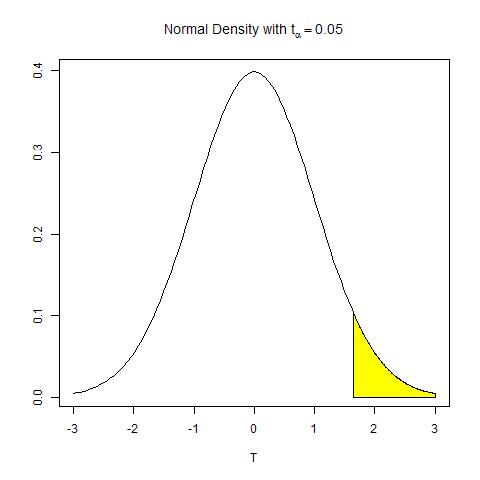
\includegraphics[width=\textwidth,height=3.125in]{./Fig/t_alpha2.jpg}
\caption{右尾檢定圖}
\end{figure}

\begin{itemize}
\tightlist
\item
  上面的圖顯示右尾的拒斥區域等於 5\%,T=1.69。
\end{itemize}

\begin{Shaded}
\begin{Highlighting}[]
\NormalTok{alpha=}\FloatTok{0.05}
\KeywordTok{qt}\NormalTok{(}\DecValTok{1}\OperatorTok{-}\NormalTok{alpha, }\DataTypeTok{df=}\DecValTok{29}\NormalTok{)}
\CommentTok{## [1] 1.699127}
\end{Highlighting}
\end{Shaded}

\hypertarget{ux7bc4ux4f8b1}{%
\subsubsection{範例1}\label{ux7bc4ux4f8b1}}

\begin{itemize}
\item
  在 \textbf{UsingR::babies}
  這筆資料中,有父親的身高資料。請問父親的平均身高顯著高於68英吋(約172公分)嗎?還是隨機誤差?請先扣掉99這個遺漏值。
\item
  因為我們感興趣的是父親身高是否高於68英吋,至於有多高並不是重點,所以我們要進行左尾的單尾檢定,對立假設是\(\mu >68\),虛無假設則是:
\end{itemize}

\[\text{H}_{\text{0}}: \mu \leq 68\]

\begin{itemize}
\tightlist
\item
  對立假設是
\end{itemize}

\[\text{H}_{\text{1}}:\mu > 68 \]

\begin{itemize}
\tightlist
\item
  用\texttt{R}進行左尾的單尾檢定假設時,設定\(\mu\)等於\(\mu_{0}\),而且\(\textbf{alternative}='greater'\)。
\end{itemize}

\begin{Shaded}
\begin{Highlighting}[]
\NormalTok{x <-}\StringTok{ }\NormalTok{UsingR}\OperatorTok{::}\NormalTok{babies}\OperatorTok{$}\NormalTok{dht}
\NormalTok{x <-}\StringTok{ }\NormalTok{x[x}\OperatorTok{<}\DecValTok{99}\NormalTok{]}
\KeywordTok{t.test}\NormalTok{(x, }\DataTypeTok{mu=}\DecValTok{68}\NormalTok{, }\DataTypeTok{alternative=}\StringTok{"greater"}\NormalTok{)}
\CommentTok{## }
\CommentTok{##  One Sample t-test}
\CommentTok{## }
\CommentTok{## data:  x}
\CommentTok{## t = 20.796, df = 743, p-value < 2.2e-16}
\CommentTok{## alternative hypothesis: true mean is greater than 68}
\CommentTok{## 95 percent confidence interval:}
\CommentTok{##  70.02973      Inf}
\CommentTok{## sample estimates:}
\CommentTok{## mean of x }
\CommentTok{##   70.2043}
\end{Highlighting}
\end{Shaded}

\begin{itemize}
\item
  結果顯示,平均值為70.2,95\%信賴區間的左尾臨界值是70.02,高於68英吋,\(p\)值小於0.05,也就是說抽到的樣本其平均值會小於68的機會非常小。換句話說,我們拒斥虛無假設,並且結論父親的平均身高高於68英吋。
\item
  我們也可以手動計算
\end{itemize}

\begin{enumerate}
\def\labelenumi{\arabic{enumi}.}
\tightlist
\item
  以\(\bar{X}\)為檢定統計量,上面已知\(\bar{X}=70.2043\)。
\item
  計算\(Z\)值
\end{enumerate}

\[Z=\frac{\bar{X}-\mu_{0}}{S/\sqrt{n}}\]

\begin{Shaded}
\begin{Highlighting}[]
\NormalTok{x <-}\StringTok{ }\NormalTok{UsingR}\OperatorTok{::}\NormalTok{babies}\OperatorTok{$}\NormalTok{dht}
\NormalTok{x <-}\StringTok{ }\NormalTok{x[x}\OperatorTok{<}\DecValTok{99}\NormalTok{]}
\NormalTok{n=}\KeywordTok{length}\NormalTok{(x); }\KeywordTok{cat}\NormalTok{(}\StringTok{"n="}\NormalTok{,n, }\StringTok{"}\CharTok{\textbackslash{}n}\StringTok{"}\NormalTok{)}
\CommentTok{## n= 744}
\KeywordTok{cat}\NormalTok{(}\StringTok{'SD='}\NormalTok{, }\KeywordTok{sd}\NormalTok{(x), }\StringTok{'}\CharTok{\textbackslash{}n}\StringTok{'}\NormalTok{)}
\CommentTok{## SD= 2.891242}
\NormalTok{mean.x=}\KeywordTok{mean}\NormalTok{(x)}
\KeywordTok{cat}\NormalTok{(}\StringTok{'Z='}\NormalTok{, (mean.x}\DecValTok{-68}\NormalTok{)}\OperatorTok{/}\NormalTok{(}\KeywordTok{sd}\NormalTok{(x)}\OperatorTok{/}\KeywordTok{sqrt}\NormalTok{(n)),}\StringTok{'}\CharTok{\textbackslash{}n}\StringTok{'}\NormalTok{)}
\CommentTok{## Z= 20.79567}
\end{Highlighting}
\end{Shaded}

\begin{itemize}
\tightlist
\item
  計算出來\(Z\)值為20.79。接下來用\textbf{pnorm()}計算\(p\)值。
\end{itemize}

\begin{Shaded}
\begin{Highlighting}[]
\KeywordTok{pnorm}\NormalTok{(}\FloatTok{20.79}\NormalTok{)}
\CommentTok{## [1] 1}
\end{Highlighting}
\end{Shaded}

\begin{itemize}
\tightlist
\item
  結果顯示,\(p\)值等於1,表示母體參數高於68的機會為1。我們用機率密度圖表示資料的分佈、平均值以及左尾的臨界點。
\end{itemize}

\begin{Shaded}
\begin{Highlighting}[]
\NormalTok{dht <-}\StringTok{ }\NormalTok{UsingR}\OperatorTok{::}\NormalTok{babies}\OperatorTok{$}\NormalTok{dht}
\NormalTok{dht <-}\StringTok{ }\NormalTok{dht[dht}\OperatorTok{<}\DecValTok{99}\NormalTok{]}
\NormalTok{Test<-}\KeywordTok{t.test}\NormalTok{(dht, }\DataTypeTok{mu=}\DecValTok{68}\NormalTok{, }\DataTypeTok{alternative=}\StringTok{"greater"}\NormalTok{)}
\NormalTok{upper=Test}\OperatorTok{$}\NormalTok{conf.int[}\DecValTok{2}\NormalTok{]}
\NormalTok{lower=Test}\OperatorTok{$}\NormalTok{conf.int[}\DecValTok{1}\NormalTok{]}
\KeywordTok{tibble}\NormalTok{(dht) }\OperatorTok
\StringTok{  }\KeywordTok{ggplot}\NormalTok{(}\KeywordTok{aes}\NormalTok{(}\DataTypeTok{x=}\NormalTok{dht)) }\OperatorTok{+}
\StringTok{  }\CommentTok{#geom_histogram(fill='gray90') +}
\StringTok{  }\KeywordTok{geom_density}\NormalTok{(}\DataTypeTok{col=}\StringTok{'#0011EE'}\NormalTok{) }\OperatorTok{+}
\StringTok{  }\KeywordTok{geom_vline}\NormalTok{(}\DataTypeTok{xintercept =}\NormalTok{ lower, }\DataTypeTok{lty=}\DecValTok{2}\NormalTok{, }\DataTypeTok{col=}\StringTok{"#EE00AA"}\NormalTok{) }\OperatorTok{+}
\StringTok{  }\KeywordTok{geom_vline}\NormalTok{(}\DataTypeTok{xintercept =} \KeywordTok{mean}\NormalTok{(dht), }\DataTypeTok{col=}\StringTok{'#AA1100'}\NormalTok{) }\OperatorTok{+}
\StringTok{  }\KeywordTok{theme_bw}\NormalTok{()}
\end{Highlighting}
\end{Shaded}

\begin{figure}

\includegraphics{Lec_test_05052020_files/figure-latex/unnamed-chunk-31-1} \hfill{}

\caption{\label{fig:lefttailexample}左尾檢定圖}\label{fig:unnamed-chunk-31}
\end{figure}

\hypertarget{ux7bc4ux4f8b2}{%
\subsubsection{範例2}\label{ux7bc4ux4f8b2}}

\begin{itemize}
\tightlist
\item
  某家飲料工廠想要知道裝瓶的飲料是否符合包裝所標示的500ml,抽出20瓶測量其體積如下(參考\href{http://www.instantr.com/2012/12/29/performing-a-one-sample-t-test-in-r/}{Sarah
  Stowell}):
\end{itemize}

\begin{Shaded}
\begin{Highlighting}[]
\NormalTok{volume<-}\KeywordTok{c}\NormalTok{(}\FloatTok{484.11}\NormalTok{,}\FloatTok{459.49}\NormalTok{,}\FloatTok{471.38}\NormalTok{,}\FloatTok{512.01}\NormalTok{,}\FloatTok{494.48}\NormalTok{,}\FloatTok{528.63}\NormalTok{,}
  \FloatTok{493.64}\NormalTok{,}\FloatTok{485.03}\NormalTok{,}\FloatTok{473.88}\NormalTok{,}\FloatTok{501.59}\NormalTok{,}\FloatTok{502.85}\NormalTok{,}\FloatTok{538.08}\NormalTok{,}\FloatTok{465.68}\NormalTok{,}
  \FloatTok{495.03}\NormalTok{,}\FloatTok{475.32}\NormalTok{,}\FloatTok{529.41}\NormalTok{,}\FloatTok{518.13}\NormalTok{,}\FloatTok{464.32}\NormalTok{,}\FloatTok{449.08}\NormalTok{,}\FloatTok{489.27}\NormalTok{)}
\end{Highlighting}
\end{Shaded}

\begin{itemize}
\item
  因為我們感興趣的是樣本平均值是否小於500ml,所以進行右尾的單尾檢定,也就是虛無假設是樣本平均值應該等於或大於500ml。
\item
  以\texttt{R}進行\(t\)檢定
\end{itemize}

\begin{Shaded}
\begin{Highlighting}[]
\KeywordTok{t.test}\NormalTok{(volume, }\DataTypeTok{mu=}\DecValTok{500}\NormalTok{, }\DataTypeTok{alternative=}\StringTok{"less"}\NormalTok{, }
       \DataTypeTok{conf.level=}\FloatTok{0.95}\NormalTok{)}
\CommentTok{## }
\CommentTok{##  One Sample t-test}
\CommentTok{## }
\CommentTok{## data:  volume}
\CommentTok{## t = -1.5205, df = 19, p-value = 0.07243}
\CommentTok{## alternative hypothesis: true mean is less than 500}
\CommentTok{## 95 percent confidence interval:}
\CommentTok{##      -Inf 501.1569}
\CommentTok{## sample estimates:}
\CommentTok{## mean of x }
\CommentTok{##  491.5705}
\end{Highlighting}
\end{Shaded}

\begin{itemize}
\item
  結果顯示,樣本平均值為491.6。95\%的區間估計顯示,母體平均值有可能小於501,但不見得小於500。因為\(p\)值為0.07,所以當從\(\mu=500\)的母體抽樣,要抽到平均值大於500的樣本的機會是7\%,大於我們設定的5\%。換句話說,我們無法拒斥樣本平均值應該等於或大於500ml的虛無假設。
\item
  圖 \ref{fig:ggstathist}
  顯示,\(p=0.140\),這是因為進行雙尾檢定,\(p\)值會比較大。而95\%的區間估計為(480,
  504),包含了樣本平均值491以及500,顯示兩者差異不大,都落在95\%的區間內。
\end{itemize}

\begin{Shaded}
\begin{Highlighting}[]
\CommentTok{# for reproducibility}
\KeywordTok{set.seed}\NormalTok{(}\DecValTok{123}\NormalTok{)}

\CommentTok{# plot}
\KeywordTok{tibble}\NormalTok{(volume) }\OperatorTok
\NormalTok{ggstatsplot}\OperatorTok{::}\KeywordTok{gghistostats}\NormalTok{(}
  \DataTypeTok{data =}\NormalTok{ ., }
  \DataTypeTok{x =}\NormalTok{ volume, }
  \DataTypeTok{title =} \StringTok{""}\NormalTok{, }
  \DataTypeTok{caption =} \KeywordTok{substitute}\NormalTok{(}\KeywordTok{paste}\NormalTok{(}\KeywordTok{italic}\NormalTok{(}\StringTok{"Source:"}\NormalTok{), }\StringTok{""}\NormalTok{)),}
  \DataTypeTok{type =} \StringTok{"robust"}\NormalTok{,}
  \DataTypeTok{test.value =} \DecValTok{500}\NormalTok{, }\CommentTok{# default value is 0}
  \DataTypeTok{conf.level =} \FloatTok{0.95}\NormalTok{,}
  \DataTypeTok{test.value.line =} \OtherTok{TRUE}\NormalTok{, }
  \DataTypeTok{centrality.parameter =} \StringTok{"mean"}\NormalTok{, }
  \DataTypeTok{centrality.line.args =} \KeywordTok{list}\NormalTok{(}\DataTypeTok{color =} \StringTok{"darkred"}\NormalTok{), }
  \DataTypeTok{binwidth =} \FloatTok{0.8}\NormalTok{, }\CommentTok{# binwidth value (experiment)}
  \DataTypeTok{messages =} \OtherTok{FALSE}\NormalTok{, }\CommentTok{# turn off the messages}
  \CommentTok{#ggtheme = hrbrthemes::theme_ipsum_tw(), }
  \DataTypeTok{ggstatsplot.layer =}\NormalTok{ F}
\NormalTok{)}
\end{Highlighting}
\end{Shaded}

\begin{figure}

\includegraphics{Lec_test_05052020_files/figure-latex/unnamed-chunk-34-1} \hfill{}

\caption{\label{fig:ggstathist}結合t檢定之長條圖}\label{fig:unnamed-chunk-34}
\end{figure}

\hypertarget{ux5c0fux6a23ux672cux7684ux5e73ux5747ux6578ux6aa2ux5b9a}{%
\subsection{小樣本的平均數檢定}\label{ux5c0fux6a23ux672cux7684ux5e73ux5747ux6578ux6aa2ux5b9a}}

\begin{itemize}
\tightlist
\item
  樣本小於30時,必須使用\(t\)檢定。步驟與上述的雙尾檢定以及單尾檢定一樣。
\end{itemize}

\hypertarget{ux6bcdux9ad4ux6bd4ux4f8bux7684ux6aa2ux5b9a}{%
\subsection{母體比例的檢定}\label{ux6bcdux9ad4ux6bd4ux4f8bux7684ux6aa2ux5b9a}}

\begin{itemize}
\tightlist
\item
  母體參數可能是比例\(p\),例如性別的比例、產品的不良率等等。跟區間估計一樣,檢定統計量\(Z\)或者\(T\)需要用到樣本的比例\(\hat{p}\),也就是:
\end{itemize}

\[Z=\frac{\hat{p}-p}{\text{SE}(p)}\]

其中

\[\text{SE}(p)=\sqrt{\frac{p\times(1-p)}{n}}\]

\begin{enumerate}
\def\labelenumi{\arabic{enumi}.}
\tightlist
\item
  選定樣本分配:
\end{enumerate}

\[\hat{p}\sim N(p,\frac{p(1-p)}{n})\]

\begin{enumerate}
\def\labelenumi{\arabic{enumi}.}
\setcounter{enumi}{1}
\tightlist
\item
  計算標準誤
\item
  計算檢定值
\item
  如果檢定值\textgreater0.05,則接受虛無假設。反之,則拒斥虛無假設。
\end{enumerate}

\hypertarget{ux7bc4ux4f8b-1}{%
\subsubsection{範例}\label{ux7bc4ux4f8b-1}}

\begin{itemize}
\item
  隨機抽樣1,000位大學生,其中615人表示希望繼續就讀研究所,請問所有學生就讀研究所的意願是否超過6成?
\item
  虛無假設:
\end{itemize}

\[H_{0}: P\leq 0.6\]

\begin{itemize}
\tightlist
\item
  對立假設:
\end{itemize}

\[H_{1}: P>0.6\]

\begin{itemize}
\tightlist
\item
  因為對立假設是\(P>0.6\),所以要進行右尾檢定。我們先計算\(\hat{p}\),然後計算標準誤,接著計算\(T\)值,並且計算\(p\)值。
\end{itemize}

\begin{Shaded}
\begin{Highlighting}[]
\NormalTok{phat=}\DecValTok{615}\OperatorTok{/}\DecValTok{1000}
\NormalTok{p=}\FloatTok{0.6}
\NormalTok{n=}\DecValTok{1000}
\NormalTok{se=}\KeywordTok{sqrt}\NormalTok{(p}\OperatorTok{*}\NormalTok{(}\DecValTok{1}\OperatorTok{-}\NormalTok{p)}\OperatorTok{/}\NormalTok{n)}
\NormalTok{T=(phat}\FloatTok{-0.6}\NormalTok{)}\OperatorTok{/}\NormalTok{se}
\KeywordTok{cat}\NormalTok{(}\StringTok{"T="}\NormalTok{,T)}
\CommentTok{## T= 0.9682458}
\KeywordTok{cat}\NormalTok{(}\StringTok{"P="}\NormalTok{,}\KeywordTok{pt}\NormalTok{(T, n}\DecValTok{-1}\NormalTok{, }\DataTypeTok{lower.tail =}\NormalTok{ F))}
\CommentTok{## P= 0.166578}
\end{Highlighting}
\end{Shaded}

\hypertarget{ux5169ux500bux7368ux7acbux6bcdux9ad4ux4e4bux6a23ux672cux6aa2ux5b9a}{%
\subsection{兩個獨立母體之樣本檢定}\label{ux5169ux500bux7368ux7acbux6bcdux9ad4ux4e4bux6a23ux672cux6aa2ux5b9a}}

\begin{itemize}
\item
  我們經常需要知道兩套樣本的差異是否達到統計上的顯著水準,例如兩種教學方法的成績、兩個餐廳的評價、兩個國家人民對於民主的滿意程度等等。
\item
  從兩個獨立母體抽樣,樣本的平均數差異(\(\bar{X_{1}}-\bar{X_{2}}\))的抽樣分配趨近於常態分配。
\item
  如果母體的變異數未知,只有樣本的變異數,我們可以用樣本變異數做為母體變藝術的估計。
\item
  那麼如何計算兩套樣本的標準誤?公式為:
\end{itemize}

\(SE(\bar{X_{1}}-\bar{X_{2}})=\sqrt{\frac{s_{1}^{2}}{n_{1}}+\frac{s_{1}^{2}}{n_{1}}}\)

如果\(n_{1}=n_{2}=n\),
\(SE(\bar{X_{1}}-\bar{X_{2}})=\sqrt{\frac{s_{1}^{2}+s_{2}^{2}}{n}}\)

如果兩者樣本數不相等,
\(SE(\bar{X_{1}}-\bar{X_{2}})=\frac{s_{1}+s_{2}}{2}\sqrt{\frac{1}{n_{1}}+\frac{1}{n_{2}}}\)

\begin{itemize}
\tightlist
\item
  \(T\)值的公式為:
\end{itemize}

\(T=\frac{\bar{X_{1}}-\bar{X_{2}}}{SE(\bar{X_{1}}-\bar{X_{2}})}\)

\begin{itemize}
\tightlist
\item
  自由度:\(n_{1}+n_{2}-2\)
\end{itemize}

\hypertarget{ux7bc4ux4f8b-2}{%
\subsubsection{範例}\label{ux7bc4ux4f8b-2}}

\begin{itemize}
\tightlist
\item
  假設有兩種油漆,我們想知道這兩種油漆的效果是不是相似。兩種油漆的資料如下,
\end{itemize}

\begin{Shaded}
\begin{Highlighting}[]
\NormalTok{sample1<-}\KeywordTok{c}\NormalTok{(}\FloatTok{19.7475}\NormalTok{, }\FloatTok{30.5562}\NormalTok{, }\FloatTok{11.0734}\NormalTok{, }\FloatTok{18.1730}\NormalTok{, }\FloatTok{19.8387}\NormalTok{, }
           \FloatTok{14.5291}\NormalTok{, }\FloatTok{19.4998}\NormalTok{, }\FloatTok{18.8374}\NormalTok{, }\FloatTok{12.6873}\NormalTok{, }\FloatTok{14.7627}\NormalTok{,}
           \FloatTok{18.3869}\NormalTok{, }\FloatTok{17.9287}\NormalTok{, }\FloatTok{17.6973}\NormalTok{, }\FloatTok{14.3439}\NormalTok{, }\FloatTok{10.7374}\NormalTok{, }
           \FloatTok{15.3563}\NormalTok{, }\FloatTok{19.0878}\NormalTok{, }\FloatTok{12.5745}\NormalTok{, }\FloatTok{18.0030}\NormalTok{, }\FloatTok{18.6004}\NormalTok{)}

\NormalTok{sample2<-}\KeywordTok{c}\NormalTok{(}\FloatTok{17.4715}\NormalTok{, }\FloatTok{9.8613}\NormalTok{, }\FloatTok{23.4827}\NormalTok{, }\FloatTok{13.6029}\NormalTok{, }\FloatTok{20.0386}\NormalTok{, }
           \FloatTok{19.6289}\NormalTok{, }\FloatTok{24.9357}\NormalTok{, }\FloatTok{17.8812}\NormalTok{, }\FloatTok{12.6012}\NormalTok{, }\FloatTok{9.7741}\NormalTok{, }
           \FloatTok{19.9265}\NormalTok{, }\FloatTok{16.4178}\NormalTok{, }\FloatTok{20.4401}\NormalTok{, }\FloatTok{15.1119}\NormalTok{, }\FloatTok{7.9955}\NormalTok{,}
           \FloatTok{5.1385}\NormalTok{, }\FloatTok{22.4969}\NormalTok{, }\FloatTok{17.4448}\NormalTok{, }\FloatTok{17.6675}\NormalTok{, }\FloatTok{7.0984}\NormalTok{)}
\end{Highlighting}
\end{Shaded}

\begin{itemize}
\tightlist
\item
  先用箱形圖顯示兩套樣本的分佈,可以看出第一套樣本比較集中,第二套比較分散:
\end{itemize}

\begin{Shaded}
\begin{Highlighting}[]

\NormalTok{dt=}\KeywordTok{data.frame}\NormalTok{(sample1, sample2)}
\NormalTok{dt.m <-}\StringTok{ }\KeywordTok{melt}\NormalTok{(dt) }\OperatorTok
\KeywordTok{ggplot}\NormalTok{(}\KeywordTok{aes}\NormalTok{(}\DataTypeTok{x=}\NormalTok{variable, }\DataTypeTok{y=}\NormalTok{value)) }\OperatorTok{+}
\StringTok{  }\KeywordTok{geom_boxplot}\NormalTok{()  }\OperatorTok{+}
\StringTok{   }\KeywordTok{labs}\NormalTok{(}\DataTypeTok{x=}\StringTok{"Groups"}\NormalTok{, }\DataTypeTok{y=}\StringTok{''}\NormalTok{) }\OperatorTok{+}
\StringTok{  }\KeywordTok{stat_summary}\NormalTok{(}\DataTypeTok{fun.y=}\NormalTok{mean, }\DataTypeTok{geom=}\StringTok{"point"}\NormalTok{, }\DataTypeTok{shape=}\DecValTok{16}\NormalTok{, }\DataTypeTok{size=}\DecValTok{2}\NormalTok{, }\DataTypeTok{col=}\StringTok{'red'}\NormalTok{) }
\NormalTok{dt.m}
\end{Highlighting}
\end{Shaded}

\begin{figure}

\includegraphics{Lec_test_05052020_files/figure-latex/unnamed-chunk-37-1} \hfill{}

\caption{\label{fig:boxplot1}兩套樣本的盒型圖}\label{fig:unnamed-chunk-37}
\end{figure}

\begin{itemize}
\tightlist
\item
  以t.test()檢定假設:兩筆資料的平均數相等,或者是相減等於0?
\end{itemize}

\begin{Shaded}
\begin{Highlighting}[]
 \KeywordTok{t.test}\NormalTok{(sample1, sample2, }\DataTypeTok{var.equal =}\NormalTok{ T)}
\CommentTok{## }
\CommentTok{##  Two Sample t-test}
\CommentTok{## }
\CommentTok{## data:  sample1 and sample2}
\CommentTok{## t = 0.7348, df = 38, p-value = 0.467}
\CommentTok{## alternative hypothesis: true difference in means is not equal to 0}
\CommentTok{## 95 percent confidence interval:}
\CommentTok{##  -2.053835  4.394365}
\CommentTok{## sample estimates:}
\CommentTok{## mean of x mean of y }
\CommentTok{##  17.12107  15.95080}
\end{Highlighting}
\end{Shaded}

\begin{itemize}
\item
  由以上的結果可以看出,\(p>0.05\),因此我們無法拒斥兩筆資料的平均數相等的假設。結論是兩種油漆的效果非常相近。
\item
  根據以上公式,我們再驗算一次:
\end{itemize}

\begin{Shaded}
\begin{Highlighting}[]
\NormalTok{n1<-}\KeywordTok{length}\NormalTok{(sample1); n2<-}\KeywordTok{length}\NormalTok{(sample2)}
\NormalTok{s1<-}\KeywordTok{sd}\NormalTok{(sample1); s2<-}\KeywordTok{sd}\NormalTok{(sample2)}
\NormalTok{se <-((s1}\OperatorTok{+}\NormalTok{s2)}\OperatorTok{/}\DecValTok{2}\NormalTok{)}\OperatorTok{*}\NormalTok{(}\KeywordTok{sqrt}\NormalTok{(n1}\OperatorTok{^-}\DecValTok{1}\OperatorTok{+}\NormalTok{n2}\OperatorTok{^-}\DecValTok{1}\NormalTok{))}
\NormalTok{T=(}\KeywordTok{mean}\NormalTok{(sample1)}\OperatorTok{-}\KeywordTok{mean}\NormalTok{(sample2))}\OperatorTok{/}\NormalTok{se}
\KeywordTok{cat}\NormalTok{(}\StringTok{'t ='}\NormalTok{,T, }\StringTok{'}\CharTok{\textbackslash{}n}\StringTok{'}\NormalTok{)}
\CommentTok{## t = 0.7414099}
\NormalTok{pvalue=(}\DecValTok{1}\OperatorTok{-}\KeywordTok{pt}\NormalTok{(}\FloatTok{0.74}\NormalTok{, n1}\OperatorTok{+}\NormalTok{n2}\DecValTok{-2}\NormalTok{))}\OperatorTok{*}\DecValTok{2}
\KeywordTok{cat}\NormalTok{(}\StringTok{'p value ='}\NormalTok{, pvalue)}
\CommentTok{## p value = 0.4638476}
\end{Highlighting}
\end{Shaded}

\begin{itemize}
\tightlist
\item
  除了檢驗兩個樣本有相同的平均值,也可以檢驗一個大於另一個平均值。以上面資料為例,
\end{itemize}

\begin{Shaded}
\begin{Highlighting}[]
 \KeywordTok{t.test}\NormalTok{(sample1, sample2, }\DataTypeTok{var.equal =}\NormalTok{ T, }\DataTypeTok{alternative =} \StringTok{'less'}\NormalTok{)}
\CommentTok{## }
\CommentTok{##  Two Sample t-test}
\CommentTok{## }
\CommentTok{## data:  sample1 and sample2}
\CommentTok{## t = 0.7348, df = 38, p-value = 0.7665}
\CommentTok{## alternative hypothesis: true difference in means is less than 0}
\CommentTok{## 95 percent confidence interval:}
\CommentTok{##      -Inf 3.855357}
\CommentTok{## sample estimates:}
\CommentTok{## mean of x mean of y }
\CommentTok{##  17.12107  15.95080}
\end{Highlighting}
\end{Shaded}

\begin{itemize}
\item
  可以看出\(p\geq 0.05\)。我們不拒斥第一套樣本等於第二套樣本的平均數的假設。
\item
  又或者用隨機抽樣的資料驗證第一套樣本平均值小於第二套樣本平均值。
\end{itemize}

\begin{Shaded}
\begin{Highlighting}[]
\KeywordTok{set.seed}\NormalTok{(}\DecValTok{29393091}\NormalTok{)}
\NormalTok{x=}\KeywordTok{rnorm}\NormalTok{(}\DecValTok{30}\NormalTok{)}
\KeywordTok{set.seed}\NormalTok{(}\DecValTok{116}\NormalTok{)}
\NormalTok{y=}\KeywordTok{rnorm}\NormalTok{(}\DecValTok{100}\NormalTok{, }\KeywordTok{sqrt}\NormalTok{(}\DecValTok{2}\NormalTok{), }\DecValTok{1}\NormalTok{)}
\KeywordTok{t.test}\NormalTok{(x, y, }\DataTypeTok{alternative =} \StringTok{'greater'}\NormalTok{)}
\CommentTok{## }
\CommentTok{##  Welch Two Sample t-test}
\CommentTok{## }
\CommentTok{## data:  x and y}
\CommentTok{## t = -5.4224, df = 50.425, p-value = 1}
\CommentTok{## alternative hypothesis: true difference in means is greater than 0}
\CommentTok{## 95 percent confidence interval:}
\CommentTok{##  -1.433189       Inf}
\CommentTok{## sample estimates:}
\CommentTok{## mean of x mean of y }
\CommentTok{##  0.247371  1.342228}
\end{Highlighting}
\end{Shaded}

\begin{itemize}
\tightlist
\item
  結果顯示\(p>0.05\),因此以\(\alpha=0.05\)的標準,我們不拒斥第一套樣本平均值小於第二套樣本平均值的假設。
\end{itemize}

\hypertarget{ux96d9ux6a23ux672cux7684ux6bd4ux4f8bux6aa2ux5b9a}{%
\subsection{雙樣本的比例檢定}\label{ux96d9ux6a23ux672cux7684ux6bd4ux4f8bux6aa2ux5b9a}}

\begin{itemize}
\tightlist
\item
  如果兩個樣本都是來自二項分布,那麼我們可以檢驗比例是否相同,也就是檢驗以下的虛無假設:
\end{itemize}

\[H_{0}:\mu_{1}-\mu_{2}=0\] -
如果把0換成任意數,等於是檢驗母體比例的差異是否達到某個程度。寫成:

\[H_{0}:\mu_{1}-\mu_{2}=D_{0}\]

\begin{itemize}
\tightlist
\item
  以上的雙尾檢定可以改為單尾檢定。
\end{itemize}

\#\#\#範例

\begin{itemize}
\tightlist
\item
  有一輛捷運,第一節車廂有50名乘客,第二節車廂有61人,第一節車廂有20位男性,第二節則有13位男性,請問兩節車廂有相同的男性比例嗎?用\texttt{R}計算如下:
\end{itemize}

\begin{Shaded}
\begin{Highlighting}[]
\NormalTok{x1=}\DecValTok{20}\NormalTok{; n1=}\DecValTok{50}\NormalTok{; x2=}\DecValTok{13}\NormalTok{; n2=}\DecValTok{61}
\KeywordTok{prop.test}\NormalTok{(}\KeywordTok{c}\NormalTok{(x1,x2), }\KeywordTok{c}\NormalTok{(n1, n2))}
\CommentTok{## }
\CommentTok{##  2-sample test for equality of proportions with continuity correction}
\CommentTok{## }
\CommentTok{## data:  c(x1, x2) out of c(n1, n2)}
\CommentTok{## X-squared = 3.7427, df = 1, p-value = 0.05304}
\CommentTok{## alternative hypothesis: two.sided}
\CommentTok{## 95 percent confidence interval:}
\CommentTok{##  -0.001604362  0.375374854}
\CommentTok{## sample estimates:}
\CommentTok{##    prop 1    prop 2 }
\CommentTok{## 0.4000000 0.2131148}
\end{Highlighting}
\end{Shaded}

\begin{itemize}
\tightlist
\item
  結果顯示,兩節車廂各有0.4以及0.21比例的男性。因為\(p>0.05\),因此以\(\alpha=0.05\)的標準,我們接受兩節車廂有一樣男性比例的假設。
\end{itemize}

\hypertarget{ux6210ux5c0dux6a23ux672cux6aa2ux5b9a}{%
\subsection{成對樣本檢定}\label{ux6210ux5c0dux6a23ux672cux6aa2ux5b9a}}

\begin{itemize}
\item
  前面的雙樣本檢定假定兩套樣本互相獨立,但是有不同的平均值與標準差。如果是想要確定兩個變數來自於同一套樣本,兩次測量的平均值相等,則是進行成對樣本檢定。
\item
  例如病患服用藥物前後的病況、選手接受訓練前後的表現等等,適合進行成對樣本檢定。
\item
  用\texttt{R}的t.test函數,可設定paired=T,進行成對樣本檢定,虛無假設為兩次測量的平均值相等。
\item
  例如比較民進黨候選人在台北市第2選區在2016年的立委選舉與2019年的立委補選的各里的平均得票率是否相同:
\end{itemize}

\begin{Shaded}
\begin{Highlighting}[]
\NormalTok{taipei<-}\KeywordTok{read.csv}\NormalTok{(}\StringTok{'./taipei201619.csv'}\NormalTok{, }\DataTypeTok{header=}\NormalTok{T, }\DataTypeTok{fileEncoding =} \StringTok{'BIG5'}\NormalTok{)}
\KeywordTok{library}\NormalTok{(dplyr)}
\NormalTok{taipei<-taipei }\OperatorTok\StringTok{ }
\StringTok{  }\KeywordTok{mutate}\NormalTok{(}\DataTypeTok{DPP2016.p=}\DecValTok{100}\OperatorTok{*}\NormalTok{DPP2016}\OperatorTok{/}\NormalTok{total2016, }\DataTypeTok{DPP2019.p=}\DecValTok{100}\OperatorTok{*}\NormalTok{DPP2019}\OperatorTok{/}\NormalTok{total2019)}
\KeywordTok{with}\NormalTok{(taipei, }\KeywordTok{t.test}\NormalTok{(DPP2016.p, DPP2019.p, }\DataTypeTok{paired =}\NormalTok{ T))}
\CommentTok{## }
\CommentTok{##  Paired t-test}
\CommentTok{## }
\CommentTok{## data:  DPP2016.p and DPP2019.p}
\CommentTok{## t = 25.822, df = 196, p-value < 2.2e-16}
\CommentTok{## alternative hypothesis: true difference in means is not equal to 0}
\CommentTok{## 95 percent confidence interval:}
\CommentTok{##  11.06842 12.89895}
\CommentTok{## sample estimates:}
\CommentTok{## mean of the differences }
\CommentTok{##                11.98368}
\end{Highlighting}
\end{Shaded}

\begin{itemize}
\item
  結果顯示兩者有很大的差異,拒斥兩次選舉的平均值相減等於0的假設。
\item
  為了確認這個檢定結果,我們可以畫圖顯示兩次選舉的平均值。先整理成為長資料:
\end{itemize}

\begin{Shaded}
\begin{Highlighting}[]
\NormalTok{dat<-}\StringTok{ }\NormalTok{taipei }\OperatorTok\StringTok{ }
\StringTok{       }\KeywordTok{select}\NormalTok{(}\StringTok{'2016'}\NormalTok{=}\StringTok{'DPP2016.p'}\NormalTok{, }\StringTok{'2019'}\NormalTok{=}\StringTok{'DPP2019.p'}\NormalTok{)}
\NormalTok{dat.new <-}\StringTok{ }\KeywordTok{melt}\NormalTok{(dat, }\DataTypeTok{variable.name =} \StringTok{"election"}\NormalTok{, }\DataTypeTok{value.name =} \StringTok{"DPP"}\NormalTok{) }
\CommentTok{## No id variables; using all as measure variables}
\NormalTok{dat.new <-}\StringTok{ }\NormalTok{dat.new }\OperatorTok\StringTok{ }
\StringTok{           }\KeywordTok{group_by}\NormalTok{(election) }\OperatorTok
\StringTok{           }\KeywordTok{mutate}\NormalTok{(}\DataTypeTok{grp.mean=}\KeywordTok{mean}\NormalTok{(DPP)) }\OperatorTok
\StringTok{           }\KeywordTok{mutate}\NormalTok{(}\DataTypeTok{Year=}\KeywordTok{as.factor}\NormalTok{(election))}
\end{Highlighting}
\end{Shaded}

然後使用ggplot2畫分佈圖:

\begin{Shaded}
\begin{Highlighting}[]
\KeywordTok{ggplot}\NormalTok{(dat.new, }\KeywordTok{aes}\NormalTok{(}\DataTypeTok{x=}\NormalTok{DPP, }\DataTypeTok{color=}\NormalTok{Year)) }\OperatorTok{+}
\StringTok{  }\KeywordTok{geom_density}\NormalTok{(}\DataTypeTok{position=}\StringTok{"identity"}\NormalTok{, }\DataTypeTok{alpha=}\NormalTok{.}\DecValTok{4}\NormalTok{) }\OperatorTok{+}
\StringTok{  }\KeywordTok{geom_vline}\NormalTok{(}\DataTypeTok{data=}\NormalTok{dat.new, }\KeywordTok{aes}\NormalTok{(}\DataTypeTok{xintercept=}\NormalTok{grp.mean, }\DataTypeTok{color=}\NormalTok{Year),}
             \DataTypeTok{linetype=}\StringTok{"dashed"}\NormalTok{) }\OperatorTok{+}
\StringTok{  }\KeywordTok{labs}\NormalTok{(}\DataTypeTok{x=}\StringTok{"DPP's Vote Share"}\NormalTok{, }\DataTypeTok{y=}\StringTok{""}\NormalTok{)}
\end{Highlighting}
\end{Shaded}

\begin{figure}

\includegraphics{Lec_test_05052020_files/figure-latex/unnamed-chunk-44-1} \hfill{}

\caption{\label{fig:DPP}民進黨2016大選及2019補選得票率}\label{fig:unnamed-chunk-44}
\end{figure}

\begin{itemize}
\tightlist
\item
  圖 \ref{fig:DPP}
  顯示發現民進黨候選人在台北市第二選區的兩次選舉的得票率,的確有相當不同的分佈以及集中趨勢。
\end{itemize}

\hypertarget{ux8b8aux7570ux6578ux5206ux6790}{%
\section{變異數分析}\label{ux8b8aux7570ux6578ux5206ux6790}}

\begin{itemize}
\item
  檢驗一個類別變數與其它連續變數(continuous
  variable)之間的關係,可運用One-way
  Anova(單因子變異數分析),分析類別之間是否存在平均值的差異。
\item
  Two-way
  Anova(雙因子變異數分析)則是有兩個以上的類別變數,分析類別之間是否存在連續變數的平均值的差異。
\item
  Anova分析建立在三個假設:
\end{itemize}

\begin{enumerate}
\def\labelenumi{\arabic{enumi}.}
\tightlist
\item
  類別變數與連續變數互相獨立
\item
  每一個類別內的連續變數呈常態分佈
\item
  每一個類別內的連續變數的變異數相同
\end{enumerate}

\begin{itemize}
\tightlist
\item
  Anova
  的目標是比較每一組之間的離散程度跟每一類別(或是每一組)內部的離散程度。兩者相比越小,表示組跟組之間的差異越小於每一組內部的差異,因此分組的意義也越小,類別變數與連續變數的關係也越小。反之則越大。
  組間變異(SSB, sum of square
  between)為各組的樣本數乘以組平均減總平均的平方的加總。
\end{itemize}

\(SSB=\sum n_{k}(\bar{x_{k}}-\bar{x})^2\)

\begin{itemize}
\tightlist
\item
  組內變異(SSW, sum of square within)為各組的變異數的加總。
\end{itemize}

\(SSW=\sum_{k}\sum (x_{ki}-\bar{x_{k}})^2\)

\begin{itemize}
\item
  全部的變異量等於這兩者相加: \(SST=SSB+SSW\)
\item
  每一組之間的平均離散程度用MSB(mean square
  between)表示,每一類別(或是每一組)內部的離散程度用MSW(mean square
  within)表示。計算方式為:
\end{itemize}

\(MSB=SSB/df(B) \hspace{.4cm} df(B)=k-1\)

\(MSW=SSW/df(W) \hspace{.4cm} df(W)=n-1-(k-1)=n-k\)

\(F=\frac{MSB}{MSW}\)

\begin{itemize}
\item
  使用\(F\)分佈而不是\(t\)分佈檢驗假設成立與否。英國統計學家兼生物學家羅納德·費雪(Ronald
  Aylmer Fisher)發明了\(F\)檢驗。
\item
  F 分佈的參數是兩個自由度,可畫圖 \ref{fig:fcurve} 如下:
\end{itemize}

\begin{Shaded}
\begin{Highlighting}[]
\KeywordTok{curve}\NormalTok{(}\KeywordTok{df}\NormalTok{(x, }\DataTypeTok{df1=}\DecValTok{1}\NormalTok{, }\DataTypeTok{df2=}\DecValTok{2}\NormalTok{), }\DataTypeTok{from=}\DecValTok{0}\NormalTok{, }\DataTypeTok{to=}\DecValTok{5}\NormalTok{, }\DataTypeTok{ylab=}\StringTok{''}\NormalTok{)}
\end{Highlighting}
\end{Shaded}

\begin{figure}

\includegraphics{Lec_test_05052020_files/figure-latex/unnamed-chunk-45-1} \hfill{}

\caption{\label{fig:fcurve}三種F分佈}\label{fig:unnamed-chunk-451}
\end{figure}

\begin{Shaded}
\begin{Highlighting}[]
\KeywordTok{curve}\NormalTok{(}\KeywordTok{df}\NormalTok{(x, }\DataTypeTok{df1=}\DecValTok{5}\NormalTok{, }\DataTypeTok{df2=}\DecValTok{6}\NormalTok{), }\DataTypeTok{from=}\DecValTok{0}\NormalTok{, }\DataTypeTok{to=}\DecValTok{5}\NormalTok{, }\DataTypeTok{col=}\StringTok{'red'}\NormalTok{, }\DataTypeTok{add=}\NormalTok{T)}
\end{Highlighting}
\end{Shaded}

\begin{figure}

\includegraphics{Lec_test_05052020_files/figure-latex/unnamed-chunk-45-2} \hfill{}

\caption{\label{fig:fcurve}三種F分佈}\label{fig:unnamed-chunk-452}
\end{figure}

\begin{Shaded}
\begin{Highlighting}[]
\KeywordTok{curve}\NormalTok{(}\KeywordTok{df}\NormalTok{(x, }\DataTypeTok{df1=}\DecValTok{20}\NormalTok{, }\DataTypeTok{df2=}\DecValTok{30}\NormalTok{), }\DataTypeTok{from=}\DecValTok{0}\NormalTok{, }\DataTypeTok{to=}\DecValTok{5}\NormalTok{, }\DataTypeTok{col=}\StringTok{'blue2'}\NormalTok{, }\DataTypeTok{add=}\NormalTok{T)}
\KeywordTok{abline}\NormalTok{(}\DataTypeTok{v=}\DecValTok{1}\NormalTok{, }\DataTypeTok{lwd=}\FloatTok{1.5}\NormalTok{, }\DataTypeTok{lty=}\DecValTok{2}\NormalTok{, }\DataTypeTok{col=}\StringTok{'green2'}\NormalTok{)}
\KeywordTok{legend}\NormalTok{(}\StringTok{'topright'}\NormalTok{, }\KeywordTok{c}\NormalTok{(}\StringTok{'df=1;df=2'}\NormalTok{,}\StringTok{'df=5;df=6'}\NormalTok{,}
                     \StringTok{'df=20;df=30'}\NormalTok{),}
            \DataTypeTok{col=}\KeywordTok{c}\NormalTok{(}\StringTok{'black'}\NormalTok{,}\StringTok{"red"}\NormalTok{, }\StringTok{"blue2"}\NormalTok{),}
            \DataTypeTok{lty=}\KeywordTok{c}\NormalTok{(}\DecValTok{1}\NormalTok{,}\DecValTok{1}\NormalTok{,}\DecValTok{1}\NormalTok{))}
\end{Highlighting}
\end{Shaded}

\begin{figure}

\includegraphics{Lec_test_05052020_files/figure-latex/unnamed-chunk-45-3} \hfill{}

\caption{\label{fig:fcurve}三種F分佈}\label{fig:unnamed-chunk-453}
\end{figure}

\begin{itemize}
\item
  圖片顯示自由度越大、\(F\)分佈圖形越接近常態分佈。
\item
  \texttt{R}的\(F\)分佈有以下指令:
\item
  df(x, df1, df1)回傳x百分比的機率 (y軸的高度)
\item
  pf(q, df1, df1)回傳q百分比的累積機率
\item
  qf(p, df1, df1)回傳p值的\(F\)值
\item
  rf(n, df1, df1)回傳從\(F\)分佈抽樣的n個樣本
\item
  以Orange這筆資料為例,我們想檢驗每一種類型的樹的樹圍是否相等。先整理資料,計算平均樹圍以及標準差:
\end{itemize}

\begin{Shaded}
\begin{Highlighting}[]
\NormalTok{Orange}\OperatorTok{$}\NormalTok{tree<-}\KeywordTok{factor}\NormalTok{(Orange}\OperatorTok{$}\NormalTok{Tree, }\DataTypeTok{levels=}\KeywordTok{c}\NormalTok{(}\StringTok{"1"}\NormalTok{,}\StringTok{"2"}\NormalTok{, }\StringTok{"3"}\NormalTok{, }\StringTok{"4"}\NormalTok{,}\StringTok{"5"}\NormalTok{))}
\KeywordTok{library}\NormalTok{(dplyr)}
\NormalTok{mydata <-}\StringTok{ }\NormalTok{Orange }\OperatorTok
\StringTok{          }\KeywordTok{group_by}\NormalTok{ (tree) }\OperatorTok
\StringTok{          }\KeywordTok{summarize}\NormalTok{(}
         \DataTypeTok{count =} \KeywordTok{n}\NormalTok{(),}
         \DataTypeTok{avg =} \KeywordTok{mean}\NormalTok{(circumference, }\DataTypeTok{na.rm =} \OtherTok{TRUE}\NormalTok{),}
         \DataTypeTok{sd =} \KeywordTok{sd}\NormalTok{(circumference, }\DataTypeTok{na.rm =} \OtherTok{TRUE}\NormalTok{)}
\NormalTok{  ) }
\KeywordTok{kable}\NormalTok{(mydata) }\OperatorTok
\StringTok{  }\KeywordTok{kable_styling}\NormalTok{(}\DataTypeTok{bootstrap_options =} \StringTok{"striped"}\NormalTok{, }\DataTypeTok{full_width =}\NormalTok{ F)}
\end{Highlighting}
\end{Shaded}

\begin{table}[H]
\centering
\begin{tabular}{l|r|r|r}
\hline
tree & count & avg & sd\\
\hline
1 & 7 & 99.57143 & 43.29302\\
\hline
2 & 7 & 135.28571 & 66.32424\\
\hline
3 & 7 & 94.00000 & 42.98062\\
\hline
4 & 7 & 139.28571 & 71.89741\\
\hline
5 & 7 & 111.14286 & 58.85980\\
\hline
\end{tabular}
\end{table}

\begin{itemize}
\item
  可以看出五種平均樹圍之間有一些差異。
\item
  用箱形圖 \ref{fig:orange} 檢視五種類型的樹圍:
\end{itemize}

\begin{Shaded}
\begin{Highlighting}[]
\NormalTok{p=}\KeywordTok{ggplot}\NormalTok{(Orange, }\KeywordTok{aes}\NormalTok{(}\DataTypeTok{x=}\NormalTok{tree, }\DataTypeTok{y=}\NormalTok{circumference)) }
\NormalTok{p}\OperatorTok{+}\KeywordTok{geom_boxplot}\NormalTok{(}\DataTypeTok{data=}\NormalTok{Orange, }\KeywordTok{aes}\NormalTok{(}\DataTypeTok{color=}\NormalTok{tree)) }\OperatorTok{+}
\StringTok{  }\KeywordTok{theme_bw}\NormalTok{()}
\end{Highlighting}
\end{Shaded}

\begin{figure}

\includegraphics{Lec_test_05052020_files/figure-latex/unnamed-chunk-47-1} \hfill{}

\caption{\label{fig:orange}五種樹的樹圍}\label{fig:unnamed-chunk-47}
\end{figure}

\begin{itemize}
\tightlist
\item
  箱形圖顯示平均數可能不相等。再用密度圖觀察是否常態分佈?
\end{itemize}

\begin{Shaded}
\begin{Highlighting}[]
\NormalTok{G=}\KeywordTok{ggplot}\NormalTok{(Orange, }\KeywordTok{aes}\NormalTok{(}\DataTypeTok{x=}\NormalTok{circumference, }\DataTypeTok{fill=}\NormalTok{tree, }\DataTypeTok{alpha=}\FloatTok{0.2}\NormalTok{))}
\NormalTok{G}\OperatorTok{+}\KeywordTok{geom_density}\NormalTok{() }\OperatorTok{+}
\StringTok{   }\KeywordTok{xlim}\NormalTok{(}\KeywordTok{c}\NormalTok{(}\DecValTok{0}\NormalTok{, }\DecValTok{300}\NormalTok{)) }\OperatorTok{+}
\StringTok{   }\KeywordTok{theme_bw}\NormalTok{()}
\end{Highlighting}
\end{Shaded}

\begin{figure}

\includegraphics{Lec_test_05052020_files/figure-latex/unnamed-chunk-48-1} \hfill{}

\caption{\label{fig:boxden}箱型圖與機率密度}\label{fig:unnamed-chunk-48}
\end{figure}

\begin{itemize}
\item
  圖 \ref{fig:boxden}
  顯示部分類別可能不是成常態分佈,而且離散程度可能不相等。
\item
  最後用aov函數進行Anova分析:
\end{itemize}

\begin{Shaded}
\begin{Highlighting}[]
\NormalTok{res.aov <-}\StringTok{ }\KeywordTok{aov}\NormalTok{(circumference }\OperatorTok{~}\StringTok{ }\NormalTok{tree, }\DataTypeTok{data =}\NormalTok{ Orange)}
\CommentTok{# Summary of the analysis}
\KeywordTok{summary}\NormalTok{(res.aov)}
\CommentTok{##             Df Sum Sq Mean Sq F value Pr(>F)}
\CommentTok{## tree         4  11841    2960   0.883  0.486}
\CommentTok{## Residuals   30 100525    3351}
\end{Highlighting}
\end{Shaded}

\begin{itemize}
\item
  結果顯示\(p>0.05\),無法拒斥五種平均樹圍相等的假設。
\item
  我們可以畫圖檢視變異數相等的假設:
\end{itemize}

\begin{Shaded}
\begin{Highlighting}[]
\KeywordTok{plot}\NormalTok{(res.aov, }\DecValTok{1}\NormalTok{, }\DataTypeTok{cex=}\FloatTok{1.5}\NormalTok{, }\DataTypeTok{lwd=}\FloatTok{1.5}\NormalTok{)}
\end{Highlighting}
\end{Shaded}

\begin{figure}

\includegraphics{Lec_test_05052020_files/figure-latex/unnamed-chunk-50-1} \hfill{}

\caption{\label{fig:anovaplot}變異數圖形}\label{fig:unnamed-chunk-50}
\end{figure}

\begin{itemize}
\item
  圖 \ref{fig:anovaplot}
  顯示,每一類別的平均值跟觀察值與該平均值之間的殘差(residual)並沒有明顯的關聯。因此,變異數相等的假設成立。
\item
  \texttt{R}另外提供Bartlett以及Levene兩種檢定變異數相等的函數。Bartlett檢驗的做法是:
\end{itemize}

\begin{Shaded}
\begin{Highlighting}[]
\KeywordTok{bartlett.test}\NormalTok{(circumference }\OperatorTok{~}\StringTok{ }\NormalTok{tree, }\DataTypeTok{data =}\NormalTok{ Orange)}
\CommentTok{## }
\CommentTok{##  Bartlett test of homogeneity of variances}
\CommentTok{## }
\CommentTok{## data:  circumference by tree}
\CommentTok{## Bartlett's K-squared = 2.4607, df = 4, p-value = 0.6517}
\end{Highlighting}
\end{Shaded}

\begin{itemize}
\tightlist
\item
  Levene檢驗則是:
\end{itemize}

\begin{Shaded}
\begin{Highlighting}[]
\KeywordTok{library}\NormalTok{(car)}
\KeywordTok{leveneTest}\NormalTok{(circumference }\OperatorTok{~}\StringTok{ }\NormalTok{tree, }\DataTypeTok{data =}\NormalTok{ Orange)}
\CommentTok{## Levene's Test for Homogeneity of Variance (center = median)}
\CommentTok{##       Df F value Pr(>F)}
\CommentTok{## group  4  0.5907  0.672}
\CommentTok{##       30}
\end{Highlighting}
\end{Shaded}

\begin{itemize}
\item
  兩個檢驗結果都是不拒斥變異數相等的假設。可以先進行這兩個檢驗,再進行變異數分析。
\item
  雖然我們無法拒斥每一組平均數相等的假設,但是我們仍然可以用TukeyHSD函數檢驗哪些組別之間可能有差異:
\end{itemize}

\begin{Shaded}
\begin{Highlighting}[]
\KeywordTok{TukeyHSD}\NormalTok{(res.aov)}
\CommentTok{##   Tukey multiple comparisons of means}
\CommentTok{##     95% family-wise confidence level}
\CommentTok{## }
\CommentTok{## Fit: aov(formula = circumference ~ tree, data = Orange)}
\CommentTok{## }
\CommentTok{## $tree}
\CommentTok{##           diff        lwr       upr     p adj}
\CommentTok{## 2-1  35.714286  -54.03528 125.46385 0.7765641}
\CommentTok{## 3-1  -5.571429  -95.32099  84.17813 0.9997503}
\CommentTok{## 4-1  39.714286  -50.03528 129.46385 0.7030223}
\CommentTok{## 5-1  11.571429  -78.17813 101.32099 0.9956073}
\CommentTok{## 3-2 -41.285714 -131.03528  48.46385 0.6725728}
\CommentTok{## 4-2   4.000000  -85.74956  93.74956 0.9999331}
\CommentTok{## 5-2 -24.142857 -113.89242  65.60671 0.9343443}
\CommentTok{## 4-3  45.285714  -44.46385 135.03528 0.5930257}
\CommentTok{## 5-3  17.142857  -72.60671 106.89242 0.9805850}
\CommentTok{## 5-4 -28.142857 -117.89242  61.60671 0.8909860}
\end{Highlighting}
\end{Shaded}

\begin{itemize}
\tightlist
\item
  結果發現每一組之間都沒有顯著的差異。
\end{itemize}

\hypertarget{ux6307ux4ee4ux6574ux7406}{%
\section{指令整理}\label{ux6307ux4ee4ux6574ux7406}}

\begin{itemize}
\tightlist
\item
  \(\tt{qnorm(conf, mean, sd)}\):
  已知平均數、變異數,求一定信賴水準下的Z值(\(\text{z}_{\alpha/2}\))
\end{itemize}

\begin{Shaded}
\begin{Highlighting}[]
\NormalTok{alpha=}\FloatTok{0.01}\NormalTok{; }\KeywordTok{cat}\NormalTok{(}\StringTok{"conf=0.99, mean=0, sd=1, Z="}\NormalTok{, }\KeywordTok{qnorm}\NormalTok{(}\DecValTok{1}\OperatorTok{-}\NormalTok{(alpha}\OperatorTok{/}\DecValTok{2}\NormalTok{), }\DecValTok{0}\NormalTok{, }\DecValTok{1}\NormalTok{),}\StringTok{"}\CharTok{\textbackslash{}n}\StringTok{"}\NormalTok{)}
\CommentTok{## conf=0.99, mean=0, sd=1, Z= 2.575829}
\NormalTok{alpha=}\FloatTok{0.05}\NormalTok{; }\KeywordTok{cat}\NormalTok{(}\StringTok{"conf=0.95, mean=0, sd=1, Z="}\NormalTok{, }\KeywordTok{qnorm}\NormalTok{(}\DecValTok{1}\OperatorTok{-}\NormalTok{alpha}\OperatorTok{/}\DecValTok{2}\NormalTok{),}\StringTok{"}\CharTok{\textbackslash{}n}\StringTok{"}\NormalTok{)}
\CommentTok{## conf=0.95, mean=0, sd=1, Z= 1.959964}
\NormalTok{alpha=}\FloatTok{0.1}\NormalTok{; }\KeywordTok{cat}\NormalTok{(}\StringTok{"conf=0.90, mean=0, sd=1, Z="}\NormalTok{, }\KeywordTok{qnorm}\NormalTok{(}\DecValTok{1}\OperatorTok{-}\NormalTok{alpha}\OperatorTok{/}\DecValTok{2}\NormalTok{),}\StringTok{"}\CharTok{\textbackslash{}n}\StringTok{"}\NormalTok{)}
\CommentTok{## conf=0.90, mean=0, sd=1, Z= 1.644854}
\NormalTok{alpha=}\FloatTok{0.05}\NormalTok{; }\KeywordTok{cat}\NormalTok{(}\StringTok{"conf=0.95, mean=1, sd=1, Z="}\NormalTok{, }\KeywordTok{qnorm}\NormalTok{(}\DecValTok{1}\OperatorTok{-}\NormalTok{alpha}\OperatorTok{/}\DecValTok{2}\NormalTok{, }\DecValTok{1}\NormalTok{, }\DecValTok{1}\NormalTok{),}\StringTok{"}\CharTok{\textbackslash{}n}\StringTok{"}\NormalTok{)}
\CommentTok{## conf=0.95, mean=1, sd=1, Z= 2.959964}
\end{Highlighting}
\end{Shaded}

\begin{itemize}
\tightlist
\item
  請參考圖 \ref{fig:twotailnormal}
  顯示信賴區間為0.95(\(\alpha=0.05\))的常態分佈,以及兩側各為0.025的拒斥區域。
\end{itemize}

\begin{figure}

\includegraphics{Lec_test_05052020_files/figure-latex/unnamed-chunk-55-1} \hfill{}

\caption{\label{fig:twotailnormal}信賴區間0.95常態分佈圖}\label{fig:unnamed-chunk-55}
\end{figure}

\begin{itemize}
\tightlist
\item
  \(\tt{pnorm(z, mean, sd)}\):
  已知z值,平均數、變異數,求累積機率值(\(\text{p}(Z\leq z^{*})\)),參考圖
  \ref{fig:onetail1}。
\end{itemize}

\begin{Shaded}
\begin{Highlighting}[]
\KeywordTok{cat}\NormalTok{(}\StringTok{"z=1.99, mean=0, sd=1, p="}\NormalTok{, }\KeywordTok{pnorm}\NormalTok{(}\FloatTok{1.99}\NormalTok{, }\DecValTok{0}\NormalTok{, }\DecValTok{1}\NormalTok{),}\StringTok{"}\CharTok{\textbackslash{}n}\StringTok{"}\NormalTok{)}
\CommentTok{## z=1.99, mean=0, sd=1, p= 0.9767045}
\KeywordTok{cat}\NormalTok{(}\StringTok{"z=1.96, mean=0, sd=1, p="}\NormalTok{, }\KeywordTok{pnorm}\NormalTok{(}\FloatTok{1.96}\NormalTok{, }\DecValTok{0}\NormalTok{, }\DecValTok{1}\NormalTok{),}\StringTok{"}\CharTok{\textbackslash{}n}\StringTok{"}\NormalTok{)}
\CommentTok{## z=1.96, mean=0, sd=1, p= 0.9750021}
\KeywordTok{cat}\NormalTok{(}\StringTok{"z=1.68, mean=0, sd=1, p="}\NormalTok{, }\KeywordTok{pnorm}\NormalTok{(}\FloatTok{1.68}\NormalTok{, }\DecValTok{0}\NormalTok{, }\DecValTok{1}\NormalTok{),}\StringTok{"}\CharTok{\textbackslash{}n}\StringTok{"}\NormalTok{)}
\CommentTok{## z=1.68, mean=0, sd=1, p= 0.9535213}
\end{Highlighting}
\end{Shaded}

\begin{itemize}
\tightlist
\item
  \(1-\tt{pnorm(z, mean, sd)}\):
  已知\(z^{*}\)值,平均數、變異數,求右尾機率值(\(\text{p}(Z\geq z^{*})\))
\end{itemize}

\begin{Shaded}
\begin{Highlighting}[]
\KeywordTok{cat}\NormalTok{(}\StringTok{"z=2.5, mean=0, sd=1, p="}\NormalTok{, }\DecValTok{1}\OperatorTok{-}\KeywordTok{pnorm}\NormalTok{(}\FloatTok{2.5}\NormalTok{, }\DecValTok{0}\NormalTok{, }\DecValTok{1}\NormalTok{),}\StringTok{"}\CharTok{\textbackslash{}n}\StringTok{"}\NormalTok{)}
\CommentTok{## z=2.5, mean=0, sd=1, p= 0.006209665}
\KeywordTok{cat}\NormalTok{(}\StringTok{"z=1.96, mean=0, sd=1, p="}\NormalTok{, }\DecValTok{1}\OperatorTok{-}\KeywordTok{pnorm}\NormalTok{(}\FloatTok{1.96}\NormalTok{, }\DecValTok{0}\NormalTok{, }\DecValTok{1}\NormalTok{),}\StringTok{"}\CharTok{\textbackslash{}n}\StringTok{"}\NormalTok{)}
\CommentTok{## z=1.96, mean=0, sd=1, p= 0.0249979}
\KeywordTok{cat}\NormalTok{(}\StringTok{"z=1.68, mean=0, sd=1, p="}\NormalTok{, }\DecValTok{1}\OperatorTok{-}\KeywordTok{pnorm}\NormalTok{(}\FloatTok{1.68}\NormalTok{, }\DecValTok{0}\NormalTok{, }\DecValTok{1}\NormalTok{),}\StringTok{"}\CharTok{\textbackslash{}n}\StringTok{"}\NormalTok{)}
\CommentTok{## z=1.68, mean=0, sd=1, p= 0.04647866}
\end{Highlighting}
\end{Shaded}

\begin{itemize}
\tightlist
\item
  \(\tt{qt(1-alpha/2, df)}\):
  已知自由度,求一定信賴水準下的T值(\(\text{t}_{\alpha/2}\))
\end{itemize}

\begin{Shaded}
\begin{Highlighting}[]
\NormalTok{n=}\DecValTok{10}\NormalTok{; alpha=}\FloatTok{0.01}\NormalTok{; }\KeywordTok{cat}\NormalTok{(}\StringTok{"conf=0.99, n=10, T="}\NormalTok{, }\KeywordTok{qt}\NormalTok{(}\DecValTok{1}\OperatorTok{-}\NormalTok{alpha}\OperatorTok{/}\DecValTok{2}\NormalTok{, n}\DecValTok{-1}\NormalTok{),}\StringTok{"}\CharTok{\textbackslash{}n}\StringTok{"}\NormalTok{)}
\CommentTok{## conf=0.99, n=10, T= 3.249836}
\NormalTok{n=}\DecValTok{10}\NormalTok{; alpha=}\FloatTok{0.05}\NormalTok{; }\KeywordTok{cat}\NormalTok{(}\StringTok{"conf=0.95, n=10, T="}\NormalTok{, }\KeywordTok{qt}\NormalTok{(}\DecValTok{1}\OperatorTok{-}\NormalTok{alpha}\OperatorTok{/}\DecValTok{2}\NormalTok{, n}\DecValTok{-1}\NormalTok{),}\StringTok{"}\CharTok{\textbackslash{}n}\StringTok{"}\NormalTok{)}
\CommentTok{## conf=0.95, n=10, T= 2.262157}
\NormalTok{n=}\DecValTok{10}\NormalTok{; alpha=}\FloatTok{0.1}\NormalTok{; }\KeywordTok{cat}\NormalTok{(}\StringTok{"conf=0.90,  n=10, T="}\NormalTok{, }\KeywordTok{qt}\NormalTok{(}\DecValTok{1}\OperatorTok{-}\NormalTok{alpha}\OperatorTok{/}\DecValTok{2}\NormalTok{, n}\DecValTok{-1}\NormalTok{),}\StringTok{"}\CharTok{\textbackslash{}n}\StringTok{"}\NormalTok{)}
\CommentTok{## conf=0.90,  n=10, T= 1.833113}
\NormalTok{n=}\DecValTok{30}\NormalTok{; alpha=}\FloatTok{0.05}\NormalTok{; }\KeywordTok{cat}\NormalTok{(}\StringTok{"conf=0.95, n=30, T="}\NormalTok{, }\KeywordTok{qt}\NormalTok{(}\DecValTok{1}\OperatorTok{-}\NormalTok{alpha}\OperatorTok{/}\DecValTok{2}\NormalTok{, n}\DecValTok{-1}\NormalTok{),}\StringTok{"}\CharTok{\textbackslash{}n}\StringTok{"}\NormalTok{)}
\CommentTok{## conf=0.95, n=30, T= 2.04523}
\end{Highlighting}
\end{Shaded}

\begin{itemize}
\tightlist
\item
  \(\tt{pt(t, df)}\):
  已知自由度,求累積機率值(\(\text{p}(T\leq t^{*})\))
\end{itemize}

\begin{Shaded}
\begin{Highlighting}[]
\NormalTok{n=}\DecValTok{10}\NormalTok{; alpha=}\FloatTok{0.01}\NormalTok{;}\KeywordTok{cat}\NormalTok{(}\StringTok{"t=1.99, n=10, p="}\NormalTok{, }\KeywordTok{pt}\NormalTok{(}\FloatTok{1.99}\NormalTok{, n}\DecValTok{-1}\NormalTok{),}\StringTok{"}\CharTok{\textbackslash{}n}\StringTok{"}\NormalTok{)}
\CommentTok{## t=1.99, n=10, p= 0.9611017}
\NormalTok{n=}\DecValTok{10}\NormalTok{; alpha=}\FloatTok{0.05}\NormalTok{;}\KeywordTok{cat}\NormalTok{(}\StringTok{"t=1.96, n=10, p="}\NormalTok{, }\KeywordTok{pt}\NormalTok{(}\FloatTok{1.96}\NormalTok{, n}\DecValTok{-1}\NormalTok{),}\StringTok{"}\CharTok{\textbackslash{}n}\StringTok{"}\NormalTok{)}
\CommentTok{## t=1.96, n=10, p= 0.9591778}
\NormalTok{n=}\DecValTok{10}\NormalTok{; alpha=}\FloatTok{0.1}\NormalTok{;}\KeywordTok{cat}\NormalTok{(}\StringTok{"t=1.68, n=10, p="}\NormalTok{, }\KeywordTok{pt}\NormalTok{(}\FloatTok{1.68}\NormalTok{, n}\DecValTok{-1}\NormalTok{),}\StringTok{"}\CharTok{\textbackslash{}n}\StringTok{"}\NormalTok{)}
\CommentTok{## t=1.68, n=10, p= 0.93637}
\NormalTok{n=}\DecValTok{30}\NormalTok{; alpha=}\FloatTok{0.05}\NormalTok{;}\KeywordTok{cat}\NormalTok{(}\StringTok{"t=1.68, n=30, p="}\NormalTok{, }\KeywordTok{pt}\NormalTok{(}\FloatTok{1.68}\NormalTok{, n}\DecValTok{-1}\NormalTok{),}\StringTok{"}\CharTok{\textbackslash{}n}\StringTok{"}\NormalTok{)}
\CommentTok{## t=1.68, n=30, p= 0.9481498}
\end{Highlighting}
\end{Shaded}

\begin{itemize}
\tightlist
\item
  \(\tt{pt(t, df)}\):
  已知自由度,求右尾機率值(\(\text{p}(T\geq t^{*})\))
\end{itemize}

\begin{Shaded}
\begin{Highlighting}[]
\NormalTok{n=}\DecValTok{10}\NormalTok{; alpha=}\FloatTok{0.01}\NormalTok{;}\KeywordTok{cat}\NormalTok{(}\StringTok{"t=1.99, n=10, p="}\NormalTok{, }\DecValTok{1}\OperatorTok{-}\KeywordTok{pt}\NormalTok{(}\FloatTok{1.99}\NormalTok{, n}\DecValTok{-1}\NormalTok{),}\StringTok{"}\CharTok{\textbackslash{}n}\StringTok{"}\NormalTok{)}
\CommentTok{## t=1.99, n=10, p= 0.0388983}
\NormalTok{n=}\DecValTok{10}\NormalTok{; alpha=}\FloatTok{0.05}\NormalTok{;}\KeywordTok{cat}\NormalTok{(}\StringTok{"t=1.96, n=10, p="}\NormalTok{, }\DecValTok{1}\OperatorTok{-}\KeywordTok{pt}\NormalTok{(}\FloatTok{1.96}\NormalTok{, n}\DecValTok{-1}\NormalTok{),}\StringTok{"}\CharTok{\textbackslash{}n}\StringTok{"}\NormalTok{)}
\CommentTok{## t=1.96, n=10, p= 0.0408222}
\NormalTok{n=}\DecValTok{10}\NormalTok{; alpha=}\FloatTok{0.1}\NormalTok{;}\KeywordTok{cat}\NormalTok{(}\StringTok{"t=1.68, n=10, p="}\NormalTok{, }\DecValTok{1}\OperatorTok{-}\KeywordTok{pt}\NormalTok{(}\FloatTok{1.68}\NormalTok{, n}\DecValTok{-1}\NormalTok{),}\StringTok{"}\CharTok{\textbackslash{}n}\StringTok{"}\NormalTok{)}
\CommentTok{## t=1.68, n=10, p= 0.06363004}
\NormalTok{n=}\DecValTok{30}\NormalTok{; alpha=}\FloatTok{0.05}\NormalTok{;}\KeywordTok{cat}\NormalTok{(}\StringTok{"t=1.68, n=30, p="}\NormalTok{, }\DecValTok{1}\OperatorTok{-}\KeywordTok{pt}\NormalTok{(}\FloatTok{1.68}\NormalTok{, n}\DecValTok{-1}\NormalTok{),}\StringTok{"}\CharTok{\textbackslash{}n}\StringTok{"}\NormalTok{)}
\CommentTok{## t=1.68, n=30, p= 0.05185016}
\end{Highlighting}
\end{Shaded}

\begin{itemize}
\tightlist
\item
  \(\tt{t.test()}\): 針對原始資料,計算一定信賴水準下的信賴區間
\end{itemize}

\begin{Shaded}
\begin{Highlighting}[]
\KeywordTok{set.seed}\NormalTok{(}\DecValTok{02138}\NormalTok{)}
\NormalTok{X<-}\KeywordTok{rnorm}\NormalTok{(}\DecValTok{100}\NormalTok{, }\DecValTok{0}\NormalTok{, }\DecValTok{1}\NormalTok{)}
\KeywordTok{t.test}\NormalTok{(X, }\DataTypeTok{conf.level=}\FloatTok{0.95}\NormalTok{)}
\CommentTok{## }
\CommentTok{##  One Sample t-test}
\CommentTok{## }
\CommentTok{## data:  X}
\CommentTok{## t = -0.81453, df = 99, p-value = 0.4173}
\CommentTok{## alternative hypothesis: true mean is not equal to 0}
\CommentTok{## 95 percent confidence interval:}
\CommentTok{##  -0.2794616  0.1167967}
\CommentTok{## sample estimates:}
\CommentTok{##   mean of x }
\CommentTok{## -0.08133247}
\CommentTok{#manual computing}
\NormalTok{n=}\KeywordTok{length}\NormalTok{(X)}
\NormalTok{mean.x<-}\KeywordTok{mean}\NormalTok{(X)}
\NormalTok{SD <-}\StringTok{ }\KeywordTok{sqrt}\NormalTok{(}\KeywordTok{var}\NormalTok{(X)}\OperatorTok{/}\NormalTok{n)}
\NormalTok{alpha=}\FloatTok{0.05}
\NormalTok{zstar<-}\KeywordTok{qnorm}\NormalTok{(}\DecValTok{1}\OperatorTok{-}\NormalTok{alpha}\OperatorTok{/}\DecValTok{2}\NormalTok{)}

\KeywordTok{cat}\NormalTok{(}\StringTok{"conf=0.95, interval estimate=["}\NormalTok{, mean.x}\OperatorTok{-}\NormalTok{zstar}\OperatorTok{*}\NormalTok{SD, }\StringTok{","}\NormalTok{, }
\NormalTok{         mean.x}\OperatorTok{+}\NormalTok{zstar}\OperatorTok{*}\NormalTok{SD,}\StringTok{"]"}\NormalTok{)}
\CommentTok{## conf=0.95, interval estimate=[ -0.2770399 , 0.114375 ]}
\end{Highlighting}
\end{Shaded}

\begin{itemize}
\tightlist
\item
  \(\tt{prop.test()}\):
  針對有比例的原始資料,計算一定信賴水準下的信賴區間(\(\hat{p}\pm t_{\alpha/2}\cdot \sqrt{\frac{p\times(1-p)}{n}}\))
\end{itemize}

\begin{Shaded}
\begin{Highlighting}[]
\KeywordTok{set.seed}\NormalTok{(}\DecValTok{02138}\NormalTok{)}
\NormalTok{X<-}\KeywordTok{rbinom}\NormalTok{(}\DecValTok{100}\NormalTok{, }\DecValTok{1}\NormalTok{, }\FloatTok{0.5}\NormalTok{)}\CommentTok{#randomly drawing samples from binomial distribution}
\NormalTok{n=}\KeywordTok{length}\NormalTok{(X)}
\NormalTok{s<-}\KeywordTok{length}\NormalTok{(X[X}\OperatorTok{==}\DecValTok{1}\NormalTok{])}
\KeywordTok{prop.test}\NormalTok{(s, n, }\DataTypeTok{conf.level =} \FloatTok{0.95}\NormalTok{)}
\CommentTok{## }
\CommentTok{##  1-sample proportions test with continuity correction}
\CommentTok{## }
\CommentTok{## data:  s out of n, null probability 0.5}
\CommentTok{## X-squared = 0.49, df = 1, p-value = 0.4839}
\CommentTok{## alternative hypothesis: true p is not equal to 0.5}
\CommentTok{## 95 percent confidence interval:}
\CommentTok{##  0.3608720 0.5622361}
\CommentTok{## sample estimates:}
\CommentTok{##    p }
\CommentTok{## 0.46}
\CommentTok{#manual computing}
\NormalTok{phat<-}\KeywordTok{mean}\NormalTok{(X)}
\NormalTok{SE <-}\StringTok{ }\KeywordTok{sqrt}\NormalTok{(phat}\OperatorTok{*}\NormalTok{(}\DecValTok{1}\OperatorTok{-}\NormalTok{phat)}\OperatorTok{/}\NormalTok{n)}
\NormalTok{alpha=}\FloatTok{0.05}
\NormalTok{tstar<-}\KeywordTok{qt}\NormalTok{(}\DecValTok{1}\OperatorTok{-}\NormalTok{alpha}\OperatorTok{/}\DecValTok{2}\NormalTok{, }\DataTypeTok{df=}\NormalTok{n}\DecValTok{-1}\NormalTok{)}

\KeywordTok{cat}\NormalTok{(}\StringTok{"conf=0.95, interval estimate=["}\NormalTok{, phat}\OperatorTok{-}\NormalTok{tstar}\OperatorTok{*}\NormalTok{SE, }\StringTok{","}\NormalTok{, }
\NormalTok{         phat}\OperatorTok{+}\NormalTok{tstar}\OperatorTok{*}\NormalTok{SE,}\StringTok{"]"}\NormalTok{)}
\CommentTok{## conf=0.95, interval estimate=[ 0.3611071 , 0.5588929 ]}
\end{Highlighting}
\end{Shaded}

\begin{itemize}
\tightlist
\item
  \(\tt{binom.test()}\):
  針對有成功數的二元資料,計算一定信賴水準下的信賴區間(\(\hat{p}\pm t_{\alpha/2}\cdot \sqrt{\frac{p\times(1-p)}{n}}\)),結果與\(\tt{prop.test()}\)相近。
\end{itemize}

\begin{Shaded}
\begin{Highlighting}[]
\KeywordTok{set.seed}\NormalTok{(}\DecValTok{02138}\NormalTok{)}
\NormalTok{X<-}\KeywordTok{rbinom}\NormalTok{(}\DecValTok{100}\NormalTok{, }\DecValTok{1}\NormalTok{, }\FloatTok{0.5}\NormalTok{)}\CommentTok{#randomly drawing samples from binomial distribution}
\NormalTok{n=}\KeywordTok{length}\NormalTok{(X)}
\NormalTok{s<-}\KeywordTok{length}\NormalTok{(X[X}\OperatorTok{==}\DecValTok{1}\NormalTok{])}
\KeywordTok{binom.test}\NormalTok{(s, n, }\DataTypeTok{conf.level =} \FloatTok{0.95}\NormalTok{)}
\CommentTok{## }
\CommentTok{##  Exact binomial test}
\CommentTok{## }
\CommentTok{## data:  s and n}
\CommentTok{## number of successes = 46, number of trials = 100, p-value = 0.4841}
\CommentTok{## alternative hypothesis: true probability of success is not equal to 0.5}
\CommentTok{## 95 percent confidence interval:}
\CommentTok{##  0.3598434 0.5625884}
\CommentTok{## sample estimates:}
\CommentTok{## probability of success }
\CommentTok{##                   0.46}
\end{Highlighting}
\end{Shaded}

\hypertarget{ux4f5cux696d}{%
\section{作業}\label{ux4f5cux696d}}

\textbf{區間估計}

\begin{enumerate}
\def\labelenumi{\arabic{enumi}.}
\item
  有一份調查的樣本數是1,000,性別的比例\(\hat{p}=0.45\)。請列出信賴水準為50\%,
  60\%, 70\%, 80\%, 95\%的區間估計。
\item
  環保署監測某個縣市的二氧化碳每小時濃度,平均值為0.36,變異數為0.16。如果二氧化碳每小時濃度成常態分佈,請問前10\%的二氧化碳每小時濃度至少是多少?
\item
  隨機抽樣調查
  350位同學,發現140位受訪者在最近一年曾經出國。請問信賴水準90\%的區間估計是甚麼?
\item
  有兩家民調公司,分別接受同一家廠商委託調查對於最新銷售的電腦的好感度。第一家公司收集\(n_{1}\)的隨機樣本,樣本變異數為\(\hat{\sigma_{1}}\)。第二家公司則認為只需要一半的隨機樣本即可,而且樣本變異數是另一家公司的四分之一,也就是\(\hat{\sigma_{2}}=0.25\hat{\sigma_{1}}\)。請回答以下子題:
\end{enumerate}

\begin{enumerate}
\def\labelenumi{(\arabic{enumi})}
\tightlist
\item
  假設第一家公司的樣本數為60,調查得到的平均為\(\hat{\mu}_{1}=34\),第二家公司調查得到的支持度為\(\hat{\mu}_{2}=39\)。請問這兩家公司對於產品好感度的最佳估計是什麼?
\end{enumerate}

(2)請問這兩家調查的支持度信賴區間分別為何?

\begin{enumerate}
\def\labelenumi{\arabic{enumi}.}
\setcounter{enumi}{4}
\item
  請畫圖檢視\(\textbf{UsingR::brightness}\) 的分佈,並且以
  \(\tt{t.test}\) 計算95\%信賴水準的區間估計。
\item
  某電商平台規定,有問題的貨品比例不能超出7\%,而倉儲抽出361個商品調查,顯示有9.5\%的貨品可能有問題。試問樣本估計的Z值為何?
\item
  續第6題,請問右尾的\(p\)值是多少?
\item
  某社區醫院統計其接生的新生兒平均重量為3千克。若隨機選擇在該醫院出生的8個嬰兒作為樣本,記錄他們的體重分別為2.8,4.0,3.3,4.1,2.9,2.8,3.2,2.76千克。請問95\%的區間估計為何?
\item
  請問\(\text{P}(0<Z<1)=?\)
\item
  隨機抽查1154位民眾,有48\%的受訪者表示應該採用電子投票,有40\%的受訪者認為應該維持紙本投票,另外有12\%沒有意見。針對電子投票的贊成比例,請問信賴水準99\%的區間估計為何?
\end{enumerate}

\textbf{假設檢定}

1. 請檢定\texttt{UsingR}中的rat這筆資料的平均數是否大於110。

2. 請問\texttt{UsingR}中的\textless span
style:``color=blue''\textgreater iq這筆資料中,iq的平均數大於100嗎?

3.
某一調查中,18位受訪者對2位候選人的表現打成績如下表,老師想知道這兩位候選人得到的成績是否相同,請問如何檢定?

\begin{table}[H]
\centering\begingroup\fontsize{14}{16}\selectfont

\begin{tabular}{r|r|r}
\hline
Respondent & Candidate.1 & Candidate.2\\
\hline
1 & 75 & 66\\
\hline
2 & 80 & 74\\
\hline
3 & 86 & 74\\
\hline
4 & 70 & 74\\
\hline
5 & 80 & 89\\
\hline
6 & 69 & 79\\
\hline
7 & 59 & 83\\
\hline
8 & 86 & 85\\
\hline
9 & 74 & 80\\
\hline
10 & 80 & 80\\
\hline
11 & 88 & 60\\
\hline
12 & 88 & 59\\
\hline
13 & 76 & 49\\
\hline
14 & 90 & 42\\
\hline
15 & 91 & 30\\
\hline
16 & 70 & 72\\
\hline
17 & 68 & 60\\
\hline
18 & 55 & 88\\
\hline
\end{tabular}
\endgroup{}
\end{table}

4.
請用Moodle上面的「立委-A05-2(台北市).ods」資料以及「候選人在各投開票所得票數一覽表」,整理台北市第二選區國民黨候選人在2016立委選舉以及2019補選的資料料,然後先畫圖比較國民黨候選人在台北市第2選區在2016年的立委選舉與2019年的立委補選的各里的分佈,最後檢驗平均得票率是否相同。

5.
請建立以下的模擬資料,然後檢驗各組的平均數是否相等。如果不相等,請找出哪兩組有不同的平均數。

\begin{Shaded}
\begin{Highlighting}[]
\KeywordTok{set.seed}\NormalTok{(}\DecValTok{377}\NormalTok{)}
\NormalTok{DV<-}\KeywordTok{rnorm}\NormalTok{(}\DecValTok{1000}\NormalTok{, }\DecValTok{0}\NormalTok{, }\DecValTok{3}\NormalTok{)}
\NormalTok{X}\FloatTok{.1}\NormalTok{<-}\KeywordTok{round}\NormalTok{(}\KeywordTok{runif}\NormalTok{(}\DecValTok{1000}\NormalTok{, }\DecValTok{1}\NormalTok{, }\DecValTok{4}\NormalTok{))}
\NormalTok{X <-}\StringTok{ }\KeywordTok{as.factor}\NormalTok{(X}\FloatTok{.1}\NormalTok{)}
\end{Highlighting}
\end{Shaded}

\begin{enumerate}
\def\labelenumi{\arabic{enumi}.}
\setcounter{enumi}{5}
\item
  某社區醫院統計其接生的新生兒平均重量為2.8千克。若隨機選擇最近一個月在該醫院出生的7個嬰兒作為樣本,記錄他們的體重分別為2.8,4.0,3.3,4.1,2.9,2.8,3.2千克。請問如果顯著水準為5\%,可否結論最近一個月出生的嬰兒平均體重等於2千8百公克?
\item
  請寫出右尾、左尾、雙尾等三種檢定的\(Z\)與\(Z_{\alpha}\)之間的關係。
\item
  \textbf{現代統計學}第10.16題第1小題。
\item
  \textbf{現代統計學}第10.18題第1小題。
\item
  \textbf{現代統計學}第10.18題第2小題。
\end{enumerate}

\hypertarget{ux66f4ux65b0ux5167ux5bb9ux65e5ux671f}{%
\section{更新內容日期}\label{ux66f4ux65b0ux5167ux5bb9ux65e5ux671f}}

\begin{verbatim}
## 最後更新日期 05/12/2020
\end{verbatim}

\end{document}
